\documentclass[11pt,a4paper,fontset=mac]{ctexart}

% ---- 版面 ----
\usepackage[a4paper,margin=2.3cm]{geometry}
\usepackage{amsmath,amssymb}
\usepackage{graphicx}
\usepackage{booktabs}
\usepackage{array}
\usepackage{caption}
\usepackage{subcaption}
\usepackage{enumitem}
\usepackage{xcolor}
\usepackage{listings}
\usepackage{multirow}
\usepackage{tikz}
\usepackage[RPvoltages]{circuitikz}
\usetikzlibrary{positioning,arrows.meta,fit,backgrounds}
\usepackage[hidelinks]{hyperref}

\captionsetup{font=small,labelfont=bf}
\setlist{itemsep=2pt,topsep=3pt,parsep=0pt}
\graphicspath{{sim/out/wave2/plots/}{sim/out/wave2/inspect/}}

\lstset{basicstyle=\ttfamily\small,breaklines=true,frame=single,
        columns=fullflexible,keepspaces=true,xleftmargin=4pt}

% 术语小框
\newcommand{\term}[1]{\textbf{#1}}

\title{\bfseries 基于接收波形的 Chiplet 晶粒间互连故障诊断\\
\large 多模态遥测的价值取决于观测的有损性}
\author{VLSI 测试课程  Mini Research Project（方向三：D2D Link 异常检测）}
\date{2026 年 6 月}

\begin{document}
\maketitle

\begin{abstract}
\noindent
异构集成（heterogeneous integration）使\term{晶粒间互连}（die-to-die, D2D）成为芯粒（chiplet）
系统的可靠性瓶颈：单封装内\term{微凸点}（micro-bump，连接相邻晶粒的微米级焊点）数以万计，
且存在大量结构测试无法预见的在役退化模式。本项目以一个纯 \texttt{ngspice}、可完全复现的
D2D 链路仿真器为数据源，构造了一个采样式操作空间的原始接收波形数据集：6000 条样本、
10 类故障（含 $15\%$ 双故障并发样本），温度、严重度、注入位置连续随机采样，发送码型逐样本
随机，并叠加信道制造偏差与发送抖动两类滋扰，在其上完成诊断、回归、消融与基线对照共六组实验。

主要结论有三。其一，原始波形上的卷积神经网络（convolutional neural network, CNN）达到
78.9\% 的十分类准确率（融合遥测 80.3\%）；而在随机码型下，直接读原始波形的逻辑回归降至
22.1\%（约等于多数类基线 20.1\%）、18 维人工眼图特征的浅层模型为 71.1\%——工作负载变化使
“从原始信号学习表征”由“略优”变为必需。其二，两类连续漂移故障的严重度回归在全部滋扰下保持
$R^2\approx0.9$。其三，也是本文的核心论点：温度与供电跌落是与真实故障征象重叠的良性混杂
因子，\textbf{多模态遥测（温度／供电跌落）的价值取决于主观测的有损程度}。模型可见完整波形时
遥测近乎冗余（$78.9\%\to80.3\%$）；而在运行时真正可得的有损标量观测（单个眼裕度）下，先知
单阈值规则在零误报工作点的故障检出率仅 46.5\%，融合温度的学习边界在同样零误报下达到 61.1\%，
并把高应力健康链路的误报率从 49\% 降到 9\%。这把“多模态融合是否有用”从定性论断变为有判决
条件的结论，也回应了课程对“人工智能（AI）何时有效、何时不必要”的要求。
\end{abstract}

% =====================================================================
\section{引言与背景}

\subsection{为什么 D2D 互连成为可靠性瓶颈}
先进制程的经济性推动系统从单片大芯片走向多芯粒解耦、再经中介层（interposer）或桥（bridge）
重新集成的形态。单封装内的 D2D 互连数量已从早期产品的不足一千升至近年高端产品的近十万，
输入／输出（I/O）密度向每平方毫米上万演进，凸点节距（pitch，相邻凸点中心间距）跌破 10\,$\mu$m。
每一根互连都要穿过微凸点、再分布层（redistribution layer, RDL）乃至硅通孔（through-silicon
via, TSV），因此一个封装拥有成千上万个相互独立的失效机会。其中相当一部分缺陷只在部署之后才
显现：电迁移、C4（受控塌陷芯片连接，controlled collapse chip connection）凸点的热机械疲劳、
晶体管阈值的负／正偏置温度不稳定性（negative/positive bias temperature instability,
NBTI/PBTI）漂移、封装翘曲诱发的成簇缺陷等。

\subsection{为什么需要在役（in-field）健康评估，而非仅靠一次性结构测试}
工业界对芯粒互连的主流测试是\term{结构测试}：通过 IEEE~1838 的晶粒包装寄存器加载确定性图案、
捕获通过／失败结果、用备用信号道修复。它严谨，但本质上是制造时的一次性活动，无法观测在役才
发展出来的弱、参数化、漂移、老化类失效——这些失效表现为时序裕度的缓慢退化而非确定的逻辑
错误，只有持续监测眼裕度、误码率、信号道偏斜的运行时监控才能捕获。

\subsection{混杂：单一健康信号天然有歧义}
D2D 链路不是孤立退化的。它的眼裕度与误码率会被\term{供电跌落}（supply droop，负载瞬变导致的
电源电压下陷）与\term{温度漂移}同时调制：一次温升或一次重负载跌落都会闭合眼图，其征象与真实
缺陷重叠。因此，要把“良性环境波动”与“萌生缺陷”区分开，本质上需要把环境共模建模并扣除——这正是
本项目要量化研究的核心问题，也是“为什么需要一个能融合多模态信号的统计模型”的根源。

% =====================================================================
\section{相关工作}\label{sec:related}

近年来，面向芯粒晶粒间互连的测试与诊断技术沿多条路线展开。基于\textbf{内建自测试}（built-in
self-test, BIST）的结构性方法利用 IEEE~1838 的晶粒包装寄存器，通过行／列条纹等确定性测试图案
检测微凸点阵列的硬开路与短路，可将测试向量数降至常数规模，并结合备用通道实现缺陷修复
~\cite{huang2024bist,chuang2025pattern,wang2024ucie}。然而，此类方法主要面向制造测试阶段，
流程依赖预定义故障模型与确定性测试图案，难以覆盖部署后出现的老化退化、环境漂移及间歇性失效等
在役故障~\cite{cui2023physical}。

随着数据驱动方法的发展，研究者开始利用 S 参数、眼图、时域反射（time-domain reflectometry, TDR）
波形以及接收端信号开展\textbf{互连故障的机器学习诊断}，采用随机森林、支持向量机、卷积神经网络
（convolutional neural network, CNN）与自编码器等模型实现故障分类与异常检测
~\cite{huang2018tsv,kang2023reflection,medico2018ae,usama2026latent}。这些工作表明机器学习能够
有效挖掘高速互连信号中的复杂特征，但大多建立在固定测试图案或受控实验环境之上，对随机工作
负载下的泛化能力缺乏系统研究；同时普遍假设可以获得完整波形或高维特征，较少考虑实际运行中观测信息
受限的情况。

针对长期可靠性，\textbf{老化监测}技术通过环形振荡器、关键路径监视器与时序传感器跟踪频率／延迟
漂移，并结合主成分分析（principal component analysis, PCA）、统计建模或机器学习预测剩余寿命
~\cite{lanzieri2024aging,ali2020fusion}；近期的片上遥测异常检测引擎进一步把多源遥测流融合为
系统级健康告警~\cite{ortega2025octane}。该类方法能反映系统整体退化趋势，但监测结果通常属于
芯片级／模块级指标，难以定位到具体互连结构或失效机理。

在\textbf{热管理}方向，热建模与电–热协同仿真工具能较准确地预测芯粒系统的温度分布与热耦合
效应~\cite{zhu2025ice,ma2024cosim}，为设计阶段的热优化与可靠性评估提供支撑；但其关注温度场分析
本身，并不面向故障诊断，更多将温度、电压等环境量视为需要补偿的外部因素，较少从诊断角度分析其与
健康征象之间的混杂耦合。

此外，部分研究从\textbf{安全可信}角度利用互连传播延迟的工艺偏差构建物理不可克隆函数（physical
unclonable function, PUF），或通过测量电源网络阻抗谱检测硬件木马与物理篡改
~\cite{deric2022puf,monfared2025quake}。这类工作验证了互连电学特征作为“指纹”的信息量，但目标
聚焦安全威胁检测，对渐进式退化与在役健康评估关注较少。

\paragraph{研究空白与本文定位。}综合现有研究：(i) 多数工作关注故障分类／缺陷检测本身，较少系统
研究温度、供电跌落等环境因素与故障征象之间的混杂关系；(ii) 普遍基于完整波形或高维特征，较少
考虑运行时观测受限（硬件开销与监测接口的限制）；(iii) 诊断模型多建立在固定激励下，对随机工作
负载场景的鲁棒性缺乏验证；(iv) 对训练未见过的新故障模式，现有分类器普遍缺乏可靠的开集识别
能力。尚无一个同时考虑运行时观测受限、环境混杂与根因诊断需求的统一框架。本文针对这四点逐一
给出可证伪的实验设计：混杂因素对所有类别同分布采样并做遥测消融（\S\ref{sec:tele}）、显式区分
完整波形与有损标量两种观测体制（\S\ref{sec:method}）、发送码型逐样本随机化并以留出码型检验
泛化（\S\ref{sec:v2ml}）、以及留一类开集实验（\S\ref{sec:openset}，诚实的负结果）。

% =====================================================================
\section{问题定义}

\paragraph{测试问题。} 给定一条 D2D 链路在某工况下采集到的接收端模拟波形，
自动判别其故障类型（10 类，含“健康”），并对连续退化故障做严重度回归；同时回答：
当运行时只能得到极有损的观测（如一个眼裕度标量）时，加入片上温度／供电跌落遥测能否抑制由良性
高应力导致的误报。

\paragraph{输入与输出。} 输入为一维接收端（RX）波形（160 个\term{单位间隔}（unit interval,
UI，一个比特占据的时间窗，本文 UI$=62.5$\,ps）$\times$ 每 UI 8 个采样 $=1280$ 点），可选叠加该
样本已知的发送比特（重建为理想发送端（TX）参考通道）与标量遥测 $[\text{温度},\text{供电跌落}]$；
输出为 10 类 softmax 概率（单故障诊断）、9 个独立故障位（多标签，覆盖并发故障，健康类对应全零）、
连续严重度（回归）、或健康／故障二分类（有损检测）之一。

\paragraph{两种观测体制（本文的关键自变量）。}
\begin{itemize}
\item \textbf{完整波形}（诊断／后硅调试态）：模型可见 1280 点全波形。对应文献中的眼图-CNN、
波形自编码器，是片上眼图监测或示波采样可达的信息上限。
\item \textbf{有损标量}（运行时真实可得）：把波形压成\textbf{单一眼裕度标量}，模拟片上裕度寄存器实际
能提供的信息。
\end{itemize}
区分这两种体制是诚实建模的要求，也是核心洞见的来源：原始模拟波形并非运行时遥测，运行时真正可得的是
有损的标量/计数。

\subsection{故障的判定：未显著恶化误码率／时延的退化算不算故障？}\label{sec:faultdef}
这是一个必须先回答的定义问题。测试理论区分四个概念：\term{缺陷}（defect，物理瑕疵）、\term{故障}
（fault，缺陷的电学/模型化表现）、\term{差错}（error，某次输出取值错误）、\term{失效}（failure，
偏离规格的可观测服务中断）。误码率（bit error rate, BER）抬升或时延越限属于差错／失效层面，而
故障是参数层面的偏离，二者不是一回事。

本文据此以“某物理／电学参数偏离其健康分布”判定故障，而非以“当前是否已造成显著 BER／时延恶化”
判定。理由有三：
\begin{enumerate}
\item \textbf{潜伏／萌生故障}（latent/incipient fault）：尚未引发误码、但已侵蚀时序与电压裕度的
退化，会在老化、温度升高或电压漂移叠加时越过阈值而失效。在役健康监测的价值正在于在其演变为
失效之前捕获它——这是本项目区别于一次性通过／失败结构测试的出发点。
\item \textbf{BER 是滞后且饱和的指标}：健康链路 BER$\approx0$，许多萌生故障要到很晚才抬升 BER
（本仿真无噪声时 BER 恒为 $10^{-300}$，故不能用作早期判据）。本文转而读波形形状并对连续故障做
严重度回归，在越限阈值以下就量化退化程度（见 \texttt{r\_drift}/\texttt{c\_drift} 的回归）。
\item \textbf{须与良性环境波动区分}：温度／供电跌落同样压低眼图却不是故障。“眼变差”不等于
“有故障”；判据是底层参数是否异常偏移，而非眼图是否变差——这正是本文混杂去除与根因分类的意义。
\end{enumerate}
\textbf{结论}：在本框架中，一个低严重度、BER 仍$\approx0$ 的 \texttt{r\_drift}/\texttt{c\_drift}/
\texttt{bump\_void\_aging} 仍算故障（潜伏态），也最值得提前检出；反之，高温下 BER 略升的健康链路
不算故障。该定义使严重度回归与混杂去除成为问题的内在组成，而非附加项。

\paragraph{为何人工智能（AI）适合。} 正常工作流形高维、且与工艺-电压-温度（process-voltage-temperature,
PVT）强相关；标注的现场失效样本稀缺；退化是渐进的。这类“学正常、判偏离 + 多模态去混杂”的问题，
与课程推荐的自编码器／长短期记忆网络（long short-term memory, LSTM）／统计异常检测同源。更具体的
“为什么必须用学习模型而不是阈值或人工特征”，将在第~\ref{sec:why} 节用专门实验回答。

% =====================================================================
\section{仿真数据源与故障建模}

\subsection{链路仿真器与电路结构}
数据源是一个纯 \texttt{ngspice}（不依赖任何商业电磁场（electromagnetic, EM）或 IBIS-AMI 链路
仿真工具）、纯标准库 Python 封装的 D2D 链路仿真器。图~\ref{fig:schematic} 给出受害信号道（victim
lane）的等效电路：行为级驱动经温度相关输出电阻 $R_\text{on}(T)$ 启动一个分段线性（piecewise-linear,
PWL）电压摆，依次穿过发送端微凸点（$R_b{+}L_b{+}C_b$）、$N{=}20$ 段 \term{RLGC 阶梯}（以电阻 $R$、
电感 $L$、电导 $G$、电容 $C$ 表征的分布参数阶梯）、接收端微凸点，到达接收节点（RX 焊盘电容
$C_\text{rx}$ 与轻终端 $R_\text{term}$）。

\term{RLGC 阶梯}指把一段分布参数传输线离散为 $N$ 个集总单元，每单元含串联电阻 $R_\text{seg}$、串联电感
$L_\text{seg}$、对地电容 $C_\text{node}$（电导 $G$ 在本短链路可忽略），用以近似传输线的频变损耗与时延。
每段取自每毫米线参数：$R'{=}0.35\,\Omega/\text{mm}$、$L'{=}0.45\,\text{nH/mm}$、$C'{=}0.18\,\text{pF/mm}$，
线长 $2\,$mm，故 $R_\text{seg}{=}0.035\,\Omega$、$L_\text{seg}{=}0.045\,$nH、$C_\text{node}{=}0.018\,$pF。
相邻两条干扰源信号道（aggressor lane）通过逐节点耦合电容 $C_c$（$C_c'{=}0.030\,$pF/mm）注入
\term{串扰}（crosstalk，邻线翻转经容性耦合在受害线上产生的噪声）。关键工艺参数取 UCIe（Universal
Chiplet Interconnect Express，通用芯粒互连标准）级短距低摆幅单端（single-ended, SE）信号：
$V_\text{dd}{=}0.8\,$V，速率 $16\,$GT/s（故 UI$=62.5\,$ps），
$Z_0{=}50\,\Omega$，导体电阻带铜温度系数 $t_{c1}{=}3.9\times10^{-3}/^\circ$C。

\begin{figure}[t]\centering
\resizebox{0.98\textwidth}{!}{%
\begin{circuitikz}[american,line width=0.7pt,every label/.style={font=\scriptsize}]
\def\gnd{-2.0}
% ---- driver ----
\draw (0,0) to[V=$v_\text{drv}$] (0,\gnd) node[ground]{};
\draw (0,0) to[R=$R_\text{on}(T)$] (2.4,0) coordinate(txo) node[above=2pt]{\scriptsize txo};
% ---- TX micro-bump (dashed box) ----
\draw[dashed,gray] (2.55,-0.6) rectangle (5.05,0.6);
\node[gray] at (3.75,0.95) {\scriptsize TX 微凸点};
\draw (txo) to[R=$R_b$] (3.75,0) to[L=$L_b$] (5.0,0) coordinate(n0) node[above=2pt]{\scriptsize n0};
\draw (n0) to[C=$C_b$] (5.0,\gnd) node[ground]{};
% ---- one RLGC segment ----
\draw (n0) to[R=$R_\text{seg}$] (6.7,0) coordinate(nm) to[L=$L_\text{seg}$] (8.3,0) coordinate(nk);
\draw (8.3,0) to[C=$C_\text{node}$] (8.3,\gnd) node[ground]{};
% coupling cap up to an aggressor rail
\draw (nm) to[C=$C_c$] (6.7,1.7) node[above]{\scriptsize 干扰源节点};
% span bracket + label BELOW the grounds (clear of every element)
\draw[gray,|-|] (5.0,-2.55) -- (8.3,-2.55);
\node[gray,below=0pt] at (6.65,-2.6) {\scriptsize $N{=}20$ 段 RLGC 阶梯};
% repetition dots in a broken span
\draw (nk) -- (8.65,0);  \draw (9.35,0) -- (9.7,0) coordinate(nN);
\node at (9.0,0) {\large$\cdots$};
% ---- RX micro-bump (dashed box) ----
\draw[dashed,gray] (9.75,-0.6) rectangle (12.25,0.6);
\node[gray] at (10.95,0.95) {\scriptsize RX 微凸点};
\draw (nN) to[R=$R_b$] (10.95,0) to[L=$L_b$] (12.2,0) coordinate(rxo) node[above=2pt]{\scriptsize rxo};
% ---- RX load (Crx to ground; Rterm to a separate mid-rail) ----
\draw (rxo) to[C=$C_\text{rx}$] (12.2,\gnd) node[ground]{};
\draw (rxo) -- (14.4,0) coordinate(rt);
\node[above] at (13.3,0.15) {\scriptsize 采样 $v$(rxo)};
\draw (rt) to[R=$R_\text{term}$] (14.4,\gnd);
\draw (14.1,\gnd) -- (14.7,\gnd);                 % mid-rail bar
\node[below=1pt] at (14.4,\gnd) {\scriptsize 中位轨 $V_\text{dd}/2$};
\end{circuitikz}}
\caption{受害信号道的 ngspice 等效电路（单端）。温度相关驱动 $R_\text{on}(T)$ 启动 PWL 摆；
信号经 TX 微凸点（$R_b{+}L_b{+}C_b$）、$N{=}20$ 段 RLGC 阶梯（逐节点对地电容 $C_\text{node}$，并经
$C_c$ 与相邻干扰源耦合）、RX 微凸点，到达接收节点（$C_\text{rx}$ + 终端 $R_\text{term}$ 接中位
电平 $V_\text{dd}/2$）。故障注入即在指定段位修改 $R_\text{seg}$、$L_\text{seg}$、$C_\text{node}$、$C_c$
或驱动摆幅（见表~\ref{tab:faultparam}）。}\label{fig:schematic}
\end{figure}

\subsection{为支撑本研究而做的四项物理扩展}
基础仿真器只能输出干净眼图，不足以表达混杂与连续退化。为此扩展四点：

\begin{enumerate}
\item \textbf{瞬态电阻热噪声。} 在受害信号道的各电阻上串入 \texttt{trnoise}（时域热电动势源），其
均方根（root mean square, RMS）正比于 $\sqrt{4k_BTR\,\Delta f}$（Johnson--Nyquist 热噪声，$k_B$ 为
玻尔兹曼常数，$T$ 温度，$R$ 电阻，$\Delta f$ 等效带宽）。物理含义：噪声随 $\sqrt{T}$ 随温度上升
（构成混杂），随 $\sqrt{R}$ 随阻性故障上升（故障自带噪声指纹）。这同时修复了无噪声时误码率恒为
$10^{-300}$ 的退化值。
\item \textbf{温度相关驱动电阻 $R_\text{on}(T)$。} 取 $R_\text{on}(T)=R_\text{on,0}\,(T/T_0)^{1.5}$（迁移率
退化）。这是温度闭合一条匹配良好短链路眼图的主导机制：本链路导体电阻仅 $0.7\,\Omega$，相对
$45\,\Omega$ 驱动电阻与 $80\,\Omega$ 终端可忽略，若不引入 $R_\text{on}(T)$，温度在波形上几乎不可观测。
引入后健康\term{眼高}（eye height，眼图睁开的垂直电压幅度）由 504\,mV 降至 419\,mV（27$\to$110$^\circ$C）。
\item \textbf{连续漂移故障与良性可观测供电跌落。} 新增 \texttt{r\_drift}（分布式串联电阻，$[15,150]\,\Omega$）
与 \texttt{c\_drift}（并联电容膨胀），作为严重度回归目标；并加入一个良性、可观测的工况供电跌落
（记入 \texttt{vdroop\_frac} 遥测列，区别于作为故障的 \texttt{supply\_droop}），作为第二个混杂因子。
\item \textbf{发送抖动（TX jitter）。} 真实链路即使健康也会因发射时钟的不完美损失时序裕量；若不建模，
“眼图闭合”就只剩故障与温度两个来源，会高估故障的可分性。实现上，为每个数据跳变沿合成一个发射时刻偏移
$\Delta t = \mathrm{RJ} + \mathrm{DCD} + \mathrm{SJ}$（随机抖动 RJ：逐沿高斯；占空比失真 DCD：上升沿
$+d/2$、下降沿 $-d/2$；周期抖动 SJ：正弦），直接加在驱动 PWL 源各跳变的时间戳上。各分量幅度逐样本
随机采样（取值范围见 \S\ref{sec:dataset}）。
\end{enumerate}

\subsection{发送/接收前端的非理想效应}\label{sec:frontend}
本数据集的前端非理想性汇总如下，它们共同决定\textbf{健康样本的眼图基线}（这也是本数据集的健康眼
低于理想发射所能达到水平的原因）：

\begin{itemize}
\item \textbf{TX 侧}：(i) 有限上升/下降沿——PWL 摆以 $t_r=0.3\,\mathrm{UI}\approx18.8\,$ps 的线性沿
发射，而非理想方波；(ii) 温度相关输出电阻 $R_\text{on}(T)=45\,\Omega\cdot(T/T_0)^{1.5}$，与信道、
终端构成分压，是温度耦合进波形的主导机制（扩展 2）；(iii) 逐沿发送抖动 RJ/DCD/SJ（扩展 4）；
(iv) 摆幅对供电跌落的乘性缩放（扩展 3）；(v) $R_\text{on}$ 的 $\pm5\%$ 逐样本制造偏差。
\item \textbf{RX 侧}：焊盘电容 $C_\text{rx}{=}30\,$fF（$\pm10\%$ 制造偏差）与接中位轨的轻终端
$R_\text{term}{=}80\,\Omega$（$\pm5\%$）构成无源负载：$C_\text{rx}$ 给出接收端的一阶带宽限制，
$R_\text{term}$ 决定直流分压并阻尼反射。
\item \textbf{未建模（边界声明）}：接收端是\textbf{无源探测}——不含连续时间线性均衡器
（continuous-time linear equalizer, CTLE）／判决反馈均衡器（decision-feedback equalizer, DFE）
均衡、判决器失调与时钟数据恢复（clock-data recovery, CDR）的采样抖动；发送端不含预加重。真实
接收机的均衡会部分重塑甚至掩盖故障征象，把诊断输入从“焊盘原始波形”变为“均衡后波形”，这是仿真到
硅的一条明确差距（见局限性）。此外，发送沿是分段线性斜坡而非晶体管的平滑（近 $\tanh$ 形）开关沿，
且 RLGC 阶梯的串阻取直流常数、不含频变损耗（趋肤效应、介质损耗）——实测信道中正是这些低通机制把
眼图棱角磨圆，故本数据集的眼图比实测硅上的更接近梯形、跳变沿更“硬”；对 $2\,$mm 短互连这一简化的
影响有限（趋肤损耗随线长累积），但属于明确的保真度边界。仿真器内置的行为级有源前端（CTLE +
tanh 判决器 + 显式供电网络（power-delivery network, PDN），见 \S\ref{sec:droopmodel}）是后续工作的
升级路径；本数据集为大批量仿真的数值稳健与可复现选用无源探测。
\end{itemize}

\subsection{故障模型：改变了哪些参数、取值范围如何}
每一类故障都对应图~\ref{fig:schematic} 中某个具体元件值的改变，并带一个明确的\textbf{严重度轴}。
表~\ref{tab:faultparam} 给出每类故障改变的参数、标称值、故障取值范围与注入位置；下文再就几类需要展开
建模的故障做说明。\term{眼裕度}（eye margin）在本文定义为有效区间内波形电平的第 90 与第 10 百分位之差，
近似眼图的垂直张开度。

\paragraph{位置术语：“段”与“节点”。}表中的注入位置沿用图~\ref{fig:schematic} 中 RLGC 阶梯的离散结构：
$2\,$mm 互连被离散为 $N{=}20$ 个串联单元，由 $21$ 个内部连接点 $n_0,\dots,n_{20}$ 隔开。
\textbf{段 $k$}（$k\in[0,19]$）指第 $k$ 个串联单元，即节点 $n_k$ 与 $n_{k+1}$ 之间的
$R_\text{seg}{+}L_\text{seg}$，物理上对应约 $0.1\,$mm 互连；段下标越小越靠近 TX 微凸点，越大越靠近 RX。
\textbf{节点 $k$}（$k\in[0,20]$）指连接点 $n_k$ 本身，其上挂有对地电容 $C_\text{node}$ 与到相邻
干扰源信号道同号节点的耦合电容 $C_c$。因此“注入段 $k$”表示修改该单元的\textbf{串联}元件
（如 \texttt{resistive\_open} 增大段串阻、\texttt{impedance\_discontinuity} 缩放段电感），
而“注入节点 $k$”表示在该连接点接入或修改\textbf{并联/耦合}元件（如 \texttt{bridge\_short}
在受害线 $n_k$ 与邻线 $n_k$ 之间接桥接电阻 $R_\text{brg}$、\texttt{crosstalk\_cap} 缩放各节点的 $C_c$）。

\begin{table}[h]\centering\footnotesize
\caption{十类故障的注入参数、标称值与取值范围。位置列中“段 $k$”（$k\in[0,19]$）指阶梯第 $k$ 个
串联单元、“节点 $k$”（$k\in[0,20]$）指第 $k$ 个连接点（定义见上文“位置术语”段），每个样本独立随机抽取。严重度均为\textbf{连续采样}：$U$ 为均匀分布，$\log U$ 为对数均匀分布
（电阻类的效应是乘性的）。\textbf{温度}：所有类别（含健康类）一律 $T\sim U(27,110)^\circ$C
连续采样，温度不构成任何类别的标签线索}\label{tab:faultparam}
\setlength{\tabcolsep}{3pt}\renewcommand{\arraystretch}{1.35}
\begin{tabular}{@{}p{2.4cm}p{3.0cm}p{1.35cm}p{4.2cm}p{2.95cm}@{}}
\toprule
类别 & 改变的参数 & 标称值 & 故障取值（连续） & 注入位置 \\
\midrule
healthy & 无注入 & —— & —— & —— \\
resistive\_\allowbreak open & 单段串阻 $+\,r_o$ & $0.035\,\Omega$ & $r_o\sim\log U(20,$ $500)\,\Omega$ & 段 $\sim U\{2,\dots,17\}$ \\
bump\_\allowbreak void\_\allowbreak aging & 单段串阻 $+\,r_o$（缓增） & $0.035\,\Omega$ & $r_o\sim\log U(5,$ $80)\,\Omega$ & 凸点端段 $\{1,2,$ $17,18\}$ \\
bridge\_\allowbreak short & 并联阻 $R_\text{brg}$ 到邻线 & 开路 & $R_\text{brg}\sim\log U(50,$ $3000)\,\Omega$ & 节点 $\sim U\{2,\dots,17\}$ \\
crosstalk\_\allowbreak cap & 耦合容 $\times f$ & $0.003\,$pF & $f\sim U(2,8)$ & 全部节点 \\
supply\_\allowbreak droop & 发送摆幅 $\times(1{-}d)$ & $0.8\,$V & $d\sim U(0.05,0.20)$ & 驱动 \\
hotspot & 5 段局部温+串阻 & 全局 $T$ & $T_\text{hot}\sim U(115,$ $160)^\circ$C & 中心段 $\sim U\{3,\dots,16\}$ $\pm2$ \\
impedance\_\allowbreak discontinuity & 3 段电感 $\times z$ & $0.045\,$nH & $z\sim U(0.4,0.75)$ $\cup\,U(1.4,3.0)$ & 起始段 $\sim U\{2,\dots,15\}$ \\
r\_\allowbreak drift & 全段串阻 $+\Delta R/N$ & $0.7\,\Omega$ 总 & $\Delta R\sim U(15,150)\,\Omega$ & 全段分布 \\
c\_\allowbreak drift & 全节点容 $\times(1{+}c)$ & $0.018\,$pF & $c\sim U(0.3,2.5)$ & 全部节点 \\
\bottomrule
\end{tabular}
\end{table}

\paragraph{阻性类（resistive\_open / bump\_void\_aging / r\_drift）。}
三者共享“串联电阻增大$\Rightarrow$分压衰减$\Rightarrow$幅度下降”的机制，区别在\textbf{空间分布与时间尺度}：
\texttt{resistive\_open} 是单段集总大阻（突发缺陷，$20$--$500\,\Omega$，约为标称段阻的 $10^3$--$10^4$ 倍）；
\texttt{bump\_void\_aging} 是同形式但幅度较小、随老化缓增（$5$--$80\,\Omega$，注入位置限于紧邻微凸点的
端部段，对应凸点空洞/电迁移的物理位置）；\texttt{r\_drift} 把总附加阻 $\Delta R$ \textbf{均分到全部 20 段}
（$R_\text{seg}\mathbin{+}{=}\Delta R/N$），表示整条线均匀老化，$\Delta R\in[15,150]\,\Omega$ 提供一条连续严重度轴。
注意 \texttt{resistive\_open} 与 \texttt{bump\_void\_aging} 的取值区间在 $20$--$80\,\Omega$ 上\textbf{有意重叠}：
两者的电学形式相同，区分线索只剩注入位置与幅度分布，这使二者构成诊断的困难对（见混淆矩阵）。

\paragraph{容性类（c\_drift / crosstalk\_cap）。} \texttt{c\_drift} 把每个对地节点电容乘 $(1{+}c)$，
$c\in[0.3,2.5]$，增大充放电时间常数$\Rightarrow$跳变沿变缓、码间串扰（inter-symbol interference,
ISI）加重，是第二条连续严重度轴；\texttt{crosstalk\_cap} 把受害线与两条干扰源间的逐节点耦合电容乘
$f\sim U(2,8)$，邻线翻转时在受害线平台／沿处注入更强的容性噪声。

\paragraph{反射类（impedance\_discontinuity）。} 在连续 3 段把段电感 $L_\text{seg}$ 乘 $z$
（$z{<}1$ 降阻抗、呈容性；$z{>}1$ 升阻抗、呈感性），形成局部特征阻抗台阶 $Z{=}\sqrt{L/C}$ 的失配。
其能量主要进入反射而非幅度衰减，故在眼图幅度上几乎不可见——这是后文区域消融中它“仅在跳变沿可检、
仅平台区时降至 0.03”的物理根源，也是单一幅度度量固有覆盖不到的一类。

\subsection{供电跌落（supply droop）的建模}\label{sec:droopmodel}
\term{供电跌落}（supply droop）指负载电流瞬变在供电网络的电阻与电感上产生压降，使驱动看到的电源
轨瞬时下陷，从而降低发送摆幅、闭合眼图。本数据集用的理想前端把它建为对发送 PWL 摆幅的乘性缩放
$V_\text{swing}\!\leftarrow\!V_\text{dd}(1{-}d)$。需区分两种供电跌落：
\begin{itemize}
\item \textbf{良性工况跌落}（混杂因子，非故障）：正常负载活动造成的可观测 IR 压降，
$d_\text{benign}\sim U(0,0.12)$ 逐样本连续采样（与噪声种子独立），记入遥测列 \texttt{vdroop\_frac}。
它像衰减类故障一样压低眼图，但属正常工况，是融合模型用来拒绝误报的依据。
\item \textbf{\texttt{supply\_droop} 故障}：一次无法由工况解释的、更大的额外跌落 $d\sim U(0.05,0.20)$，
叠加在良性跌落之上。
\end{itemize}
（仿真器另有一条行为级有源前端，把跌落建为显式供电网络：稳压源经 $R_\text{pdn}{=}20\,\text{m}\Omega$、
$L_\text{pdn}{=}100\,$pH 到去耦电容 $C_\text{dec}{=}50\,$nF，并由一个与数据相关的同步开关输出
（simultaneous switching output, SSO）电流负载真实地把电源轨拉低，产生静态 IR 压降与 $L\,di/dt$ 首跌
振铃。本研究数据集采用理想前端的等效摆幅缩放，以保证大批量仿真的数值稳健与可复现。）

\subsection{热点（hotspot）与温度的建模}
全局芯片温度 $T$ 通过 ngspice 的 \texttt{.temp} 卡作用于三处：导体电阻经铜温度系数 $t_{c1}$ 升高、
驱动输出电阻经 $R_\text{on}(T)$ 升高（主导项）、热噪声 RMS 经 $\sqrt{T}$ 升高。\texttt{healthy} 与各故障
均在 $27$--$110^\circ$C 连续均匀采样，使温度成为贯穿所有类的混杂变量而非某类的标志。

\textbf{热点故障}建模一个局部热区：在随机抽取的中心段 $\pm2$（共 5 段）把这些电阻实例的温度
钉在 $T_\text{hot}\sim U(115,160)^\circ$C（高于全局 $T$），并叠加一项随过热量增长的局部串阻
$\Delta R_\text{seg}=\max(0,(T_\text{hot}{-}90)\!\cdot\!2)/5$（模拟空洞／自热引起的电迁移退化，使该热事件在眼图上
可检）。例如 $T_\text{hot}{=}120^\circ$C 时每段加 $12\,\Omega$、五段合计 $60\,\Omega$。局部温度本身因导体阻很小
而影响有限，故热点的可观测征象主要来自这条局部串阻。

\subsection{温度与供电跌落遥测“如何被测量”}
表~\ref{tab:tele}--\ref{tab:rule} 用到的两路标量遥测，其语义与来源如下：
\begin{itemize}
\item 在\textbf{仿真}中它们是受控的潜变量：温度即每次仿真设定的 \texttt{.temp} 值（在
$27$--$110^\circ$C 上连续均匀采样），良性跌落即设定的摆幅缩减 $d_\text{benign}$；二者作为真值分别写入
数据集的 \texttt{temp\_C}、\texttt{vdroop\_frac} 两列。它们是“可测但有噪声、与故障征象重叠”的环境
共模量，而非故障标签。
\item 在\textbf{真实芯片}中它们对应成熟的片上监测电路：温度由片上数字温度传感器（digital temperature
sensor, DTS；基于双极结型晶体管（bipolar junction transistor, BJT）／二极管的热敏单元）给出；供电
跌落由片上电压跌落监测器／关键路径监测器给出。也就是说，本文“融合遥测”所需的两路信号在现代片上
系统（system on chip, SoC）中本就常态化采集，方法不依赖额外的专用探针。
\end{itemize}

\subsection{机械轴扩展（v3）：翘曲应力的电学映射与第三路遥测}\label{sec:mech}
以上多物理耦合只含\textbf{电与热}（外加供电）两个域。我们按与温度／供电跌落完全相同的逻辑补上
\textbf{机械域}：每个样本在生成前多采样一个封装应力／翘曲状态，把它映射为电学参数微扰，并额外
输出一路“应力遥测”标量——同样是受控潜变量、环境共模、写入遥测、绝不充当故障标签。
映射沿用第 3.5 节“场 $\to$ 一阶灵敏度系数 $\to$ 网表参数”的无电磁／有限元（finite-element method,
FEM）仿真方案：

\begin{enumerate}
\item \textbf{潜变量}：封装翘曲（warpage）$w\sim U(0,150)\,\mu$m 逐样本采样。总机械应力为
热膨胀系数（coefficient of thermal expansion, CTE）失配热应力与翘曲角点应力之和：
\[\sigma=\underbrace{\tfrac{E}{1-\nu}\Delta\alpha\,(T-T_0)}_{\approx 2.49\,\text{MPa}/^\circ\text{C}}
+\underbrace{k_w\,w}_{k_w=1.5\,\text{MPa}/\mu\text{m}}\in[0,\sim430]\,\text{MPa}\]
（翘曲项是曲率 $\kappa=8w/L^2$ 角点应力的标量化一阶形式）。
\item \textbf{电学映射}（三条，均为文献一阶灵敏度）：(i) \textbf{角点微凸点弹性接触电阻}（主导项）：
翘曲加载角点凸点，接触电阻可逆地增加 $\Delta R = 0.02\,\Omega/\mu\text{m}\times w$（两端各
$0$--$3\,\Omega$）——与 \texttt{bump\_void\_aging} 的\emph{永久}裂纹增长（$5$--$80\,\Omega$、单端）
机理相区分；(ii) 驱动电阻 $R_\text{on}$ 乘平均压阻因子（Smith/Kanda：$\pi_p=7.18\times10^{-4}$、
$\pi_n=3.16\times10^{-4}$/MPa，饱和区降额 0.4）——被动单电阻驱动只能携带 n 型／p 型（NMOS／PMOS）
两管的平均效应（$400$\,MPa 时约 $-3\%$），n／p 反号的应力指纹需要主动推挽前端，此处如实声明不建模；
(iii) 全部铜质电阻（走线/凸点）乘金属应变系数 $1+1.7\times10^{-5}\sigma$（$+0.7\%$ 量级，二阶项）。
\item \textbf{遥测}：新列 \texttt{stress\_MPa} $=$ CTE(全局温度) $+$ 翘曲应力，对应片上压阻应力
传感器／翘曲监测的理想化读数；与 \texttt{temp\_C} 同语义——热点的局部附加应力对它不可见。
\end{enumerate}

量级核对：健康链路 $60^\circ$C 下 $w:0\to150\,\mu$m 使眼高 $418\to386$\,mV（约 $-8\%$），与良性
跌落同量级——翘曲因此是一个真实的良性混杂（高翘曲健康链路的裕度损失可被应力遥测解释），
而其波形效应又始终低于凸点故障注入范围的下限。

\subsection{数据集：被采样的操作空间}\label{sec:dataset}
数据集规模 6000 条、每条 1280 点（160 UI $\times$ 8 样/UI），其中健康 1062 条（$17.7\%$）、
各单故障类约 470 条、双故障并发 710 条。设计原则是\textbf{采样一个操作空间，而非枚举一个网格}——
每个样本独立随机抽取以下全部因素：

\begin{enumerate}
\item \textbf{工况（混杂因子，可观测）}：温度 $T\sim U(27,110)^\circ$C、良性跌落
$d_\text{benign}\sim U(0,0.12)$，对所有类别同分布采样。这一点对混杂结论至关重要：
若某温度区间只出现某些类别，读遥测的模型会把温度当作标签捷径，遥测消融的结论便成为数据构造的
假象；同分布采样从结构上排除了这种捷径，分离健康与故障的信息只能来自（波形，遥测）的联合结构。
\item \textbf{工作负载}：受害与两条干扰源信号道的\term{伪随机比特序列}（pseudo-random bit sequence,
PRBS）种子逐样本随机——在役链路承载的是变化的任务流量而非固定图案。每个样本的发送比特随种子存入
数据集，故模型可以（可选地）以理想发送波形为条件输入，且“跳变沿区／平台区”的掩膜可逐样本重建。
\item \textbf{滋扰（影响波形但不构成标签）}：(i) \textbf{信道制造偏差}——RLGC 线参数
（$\pm8\%$）、微凸点寄生（$\pm15\%$）、$R_\text{on}$（$\pm5\%$）、$C_\text{rx}$（$\pm10\%$）、
$R_\text{term}$（$\pm5\%$）逐样本乘性扰动，防止模型指纹化单一标称信道；(ii) \textbf{发送抖动}——
随机抖动（高斯，$\sigma\sim U(0.2,1.2)$\,ps）、占空比失真（$\pm1$\,ps）与周期抖动
（幅度 $U(0,1.2)$\,ps、频率 $50$--$300$\,MHz）合成每个跳变沿的发射时刻偏移，提供故障之外的
真实眼图闭合机制。
\item \textbf{故障}：类别（健康类加权 2 倍）、连续严重度与位置按表~\ref{tab:faultparam} 采样；
$15\%$ 的故障样本叠加第二个不同类别的故障（标签为 ``a+b''），用于多标签诊断。
\end{enumerate}

生成由 8 个并行 ngspice 进程完成（约 290 次／分钟），全数据集 20.3 分钟、零仿真失败。除 8 样/UI
的重采样波形外，每次运行的完整 1\,ps 分辨率原始波形（约 $10^4$ 点）以二进制浮点格式
保留，眼高／眼宽／外推 BER 三项特征随行存储；脚本公开，无需任何工业数据。

图~\ref{fig:eyes} 给出每类故障的眼图：健康为清晰睁开的眼，阻性／供电跌落类幅度大幅下降，\texttt{c\_drift}
沿变缓，\texttt{crosstalk} 模糊，\texttt{impedance\_discontinuity} 在幅度上几乎不可见。

\begin{figure}[h]\centering

\includegraphics[width=0.92\textwidth]{eyes.png}
\caption{每类故障的接收端眼图（折叠 2 UI，由 $1\,$ps 分辨率原始波形绘制，而非机器学习输入用的
8 样／UI 重采样版本——后者每个跳变沿仅约 2.4 个采样点，画出的眼会呈折线状）。每幅子图右下角标注所叠加各次运行的眼高
$H$（最坏情形垂直开口 $\min(\text{高电平})-\max(\text{低电平})$）、眼宽 $W$
（$\mathrm{UI}$ 减峰峰抖动）与按 Q 因子高斯外推的 BER 的中位数；BER${}<10^{-30}$
表示外推值低于可显示范围（见第~\ref{sec:faultdef} 节关于 BER 饱和性的讨论）。
阻抗不连续属反射域故障，在幅度域几乎不可见，对应后文区域消融中其“仅平台区准确率 0.03”的结果。}\label{fig:eyes}
\end{figure}

% =====================================================================
\section{方法：诊断如何进行}\label{sec:method}

本节详细说明诊断的完整数据通路、模型结构、前向计算与三组消融的设计，使流程可被精确复现。

\subsection{从波形到判决的完整通路}
\begin{enumerate}[label=\textbf{步骤\arabic*.}]
\item \textbf{采集与重采样。} 对每次仿真，取受害信号道接收节点电压 $v(t)$，用线性插值重采样到统一栅格
$t_k = k\cdot(\text{UI}/8),\ k=0,\dots,1279$。统一栅格保证所有样本等长且比特相位对齐；每个样本的
发送比特由其存储的 PRBS 种子重建，区域掩膜逐样本生成。
\item \textbf{标准化。} 以训练集的全局均值与标准差对波形做 $z$-标准化（减均值、除标准差），去除数据集级的公共偏置与尺度（逐样本的相对幅度衰减得以保留），使模型关注形状。
\item \textbf{有效区裁剪。} 丢弃前 \texttt{settle\_bits} 个用于填充信道的比特，仅保留稳态有效区（1216 点）。
\item \textbf{特征提取（卷积干路）。} 见 \S\ref{sec:cnn}。
\item \textbf{判决头。} 卷积特征（可选拼接遥测）经两层多层感知机（multilayer perceptron, MLP）映射到输出 logit：单故障诊断为
10 维 softmax 取 \texttt{argmax}；多标签诊断为 9 个独立 sigmoid 位（判决阈值在验证集上按每类 F1 校准，
见 \S\ref{sec:v2ml}）；严重度回归换成单一线性输出 + 均方误差（mean squared error, MSE）。
\end{enumerate}

\subsection{卷积网络结构与前向计算}\label{sec:cnn}
诊断主模型是一维 CNN，输入为 $C\times 1216$ 波形：通道 1 是 RX 波形；可选通道 2 是由该样本
已知发送比特重建的\textbf{理想 TX 参考}（码型条件化；后文实验表明它并非必需，单通道性能相当）。
结构如下：
\begin{center}\small
$\text{Conv1d}(C\to16,k{=}7)\to\text{ReLU}\to\text{MaxPool}_2
\to\text{Conv1d}(16\to32,k{=}5)\to\text{ReLU}\to\text{MaxPool}_2
\to\text{Conv1d}(32\to64,k{=}3)\to\text{ReLU}$
\end{center}
（式中 Conv1d 为一维卷积，ReLU 为修正线性单元，MaxPool$_2$ 为步长 2 的最大池化，$k$ 为卷积核宽度。）
随后在时间维上做\textbf{平均池化与最大池化并拼接}得到 $128$ 维向量：
\[
\mathbf{f} = \big[\;\underbrace{\textstyle\frac{1}{T}\sum_t z_{:,t}}_{64\text{ 维, 均值}}\;\big\|\;
\underbrace{\max_t z_{:,t}}_{64\text{ 维, 极值}}\;\big]\quad(\big\|\text{ 表示拼接}).
\]
拼接两种池化的动机有明确物理含义：平均池化保留稳态电平／幅度指纹（阻性、供电跌落类故障的判别
信息在此），最大池化保留峰值与跳变沿信息（串扰、阻抗不连续的信息在此）。仅用全局平均池化会
把波形压成均值、丢失幅度与极值的区分——实测中这正是早期 CNN 不如线性基线的原因。
随后（若启用遥测融合）把标量遥测 $[\text{温度}/100,\ \text{供电跌落}\times10]$ 拼到 $\mathbf{f}$ 后，
经 $\text{Linear}(128(+2)\to64)\to\text{ReLU}\to\text{Linear}(64\to\text{输出维})$ 得到 logit。

\paragraph{训练细节。} 单故障十分类用带逆频率类权重的交叉熵（健康等少数类被加权），
多标签用带正例权重的二元交叉熵（binary cross-entropy, BCE）；Adam 优化器（学习率 $2\times10^{-3}$，权重衰减 $10^{-4}$），
训练 60 轮，批大小 64。数据按类别分层 75/25 划分（单故障子集训练 3967 / 测试 1323；多标签全集
4499 / 1501），随机种子固定；多标签的判决阈值在训练集内再分出的 $20\%$ 验证子集上按每类 F1 校准。

\subsection{循环网络（LSTM）对照}\label{sec:lstm}
波形本质是时间序列，因此课程推荐的另一类模型——LSTM（带门控记忆单元、沿时间逐点累积状态的循环
神经网络）——是 CNN 之外的自然选择。我们以相同的有效区波形为输入训练一个 2 层 LSTM（隐藏维 64，
沿时间每 2 个采样取 1 个以控制序列长度），取末层最后时刻的隐藏状态经同样的两层 MLP 头输出类别；
可选地在 MLP 头处拼接温度／供电跌落遥测。CNN 与 LSTM 的差异在归纳偏置：CNN 用平移不变的局部
卷积核与池化抓取“波形某处的局部形状”，LSTM 用时序递归抓取“沿时间累积的依赖”。二者对比用于检验
结论不依赖单一架构。

\subsection{对照方法}
\begin{itemize}
\item \textbf{线性基线}：多项逻辑回归，输入为标准化后的原始波形（或标量），输出为类别。它衡量“故障是否
线性可分”。
\item \textbf{人工特征基线}（\S\ref{sec:why} 新增）：不读原始波形，而是抽取 18 维标准眼图特征
（均值电平、眼裕度、标准差、平均压摆率、第 10/90 百分位，分别在全/沿/平台三区计算，区域掩膜由各
样本自己的发送比特逐行生成），训练同样的逻辑回归与一个小 MLP。它衡量“从原始信号学表征相比经典
特征工程是否更优”。
\item \textbf{单阈值规则}（\S\ref{sec:why} 新增）：有损体制下，模拟测试工程师最自然的非学习替代——
“若眼裕度 $<\tau$ 则判为故障”。
\end{itemize}

\subsection{三组消融的设计}
\begin{itemize}
\item \textbf{遥测消融}：A（仅波形）对 B（波形 + 温度／供电跌落），在两种观测体制下分别做，比较总体
准确率、高应力子集准确率、健康误报率。
\item \textbf{区域消融}：分别仅保留\textbf{沿区}（跳变沿 $\pm0.5$\,UI 窗）、仅保留\textbf{平台区}、与全波形
训练 CNN——掩膜由各样本自己的发送比特逐行生成，区域之外的采样置零——定位“故障特征住在波形何处”；
为稳健起见对每种区域做 3 次重初始化取均值$\pm$标准差。
\item \textbf{严重度回归}：在 \texttt{r\_drift}/\texttt{c\_drift} 子集上，用同一卷积干路换单输出 + MSE，
预测归一化严重度。
\end{itemize}

% =====================================================================
\section{实验结果}

\subsection{故障诊断（10 类，单故障子集，测试集 $n=1323$）}
\begin{table}[h]\centering\small
\caption{十分类诊断结果（单故障子集测试集）。多数类基线 0.201}\label{tab:diag}
\begin{tabular}{@{}lc@{}}
\toprule
模型 & 准确率 \\
\midrule
单一眼裕度标量 + 逻辑回归 & 0.221 \\
逻辑回归（原始波形） & 0.221 \\
人工眼图特征（18 维）+ 逻辑回归 & 0.661 \\
人工眼图特征（18 维）+ MLP & 0.711 \\
LSTM（原始波形） & 0.249 \\
\textbf{1-D CNN（原始波形）} & \textbf{0.789} \\
\textbf{1-D CNN + 温度／供电跌落遥测} & \textbf{0.803} \\
\bottomrule
\end{tabular}
\end{table}

表~\ref{tab:diag} 中最值得注意的一行是原始波形上的逻辑回归：0.221，与单标量持平、仅比多数类
基线高 2 个百分点。原因在码型随机化破坏了固定采样点与类别的对应关系：线性模型对每个采样维赋
一权重，而同一故障类在该维上的条件均值经各码型平均后趋于与类别无关（码型置换下的均值相消），
唯一在码型置换下不变的判别量是逐样本的整体幅度衰减（即眼裕度所编码者）——恰是一个眼裕度标量所含的信息，故线性
模型必然退化到与单标量持平。把波形压成 18 维码型不变的人工眼图特征可恢复到 0.661--0.711，但仍
比 CNN 低约 8--13 个百分点：固定的 18 维是为单类故障预设的统计量，无法同时为所有根因保留各自
依赖位置的判别量（详见 \S\ref{sec:why}），此即其信息上限。这组对照在工作负载变化下把“从原始信号
学习表征”由“略优于基线”变成必需：要么用学习的卷积特征，要么接受人工特征的信息上限。LSTM 一行
（0.249）说明这并非“任何深度模型都行”：LSTM 沿绝对时间逐点累积状态，码型随机使同一故障的局部
签名每样本落在不同比特相位，须靠长程门控重新对齐方能判别，而该对齐随码型而变、无固定权重可学；
CNN 的共享卷积核本身具备平移等变性、免去对齐，故在相同训练预算下 LSTM 接近线性模型的 0.221
水平（讨论见 \S\ref{sec:why}）。

混淆矩阵（图~\ref{fig:confusion}）的残余混淆均有物理解释：弱 \texttt{impedance\_discontinuity}
与健康类互混（$z$ 接近标称时本就几乎无电学差别）；\texttt{hotspot} 部分被判为
\texttt{resistive\_open}（二者同为局部串阻升高，热点的可观测征象正来自其局部串阻项）；
\texttt{resistive\_open} 与 \texttt{bump\_void\_aging} 在重叠的 $20$--$80\,\Omega$ 区间互混
（电学形式相同，仅位置分布不同）。

\begin{figure}[h]\centering
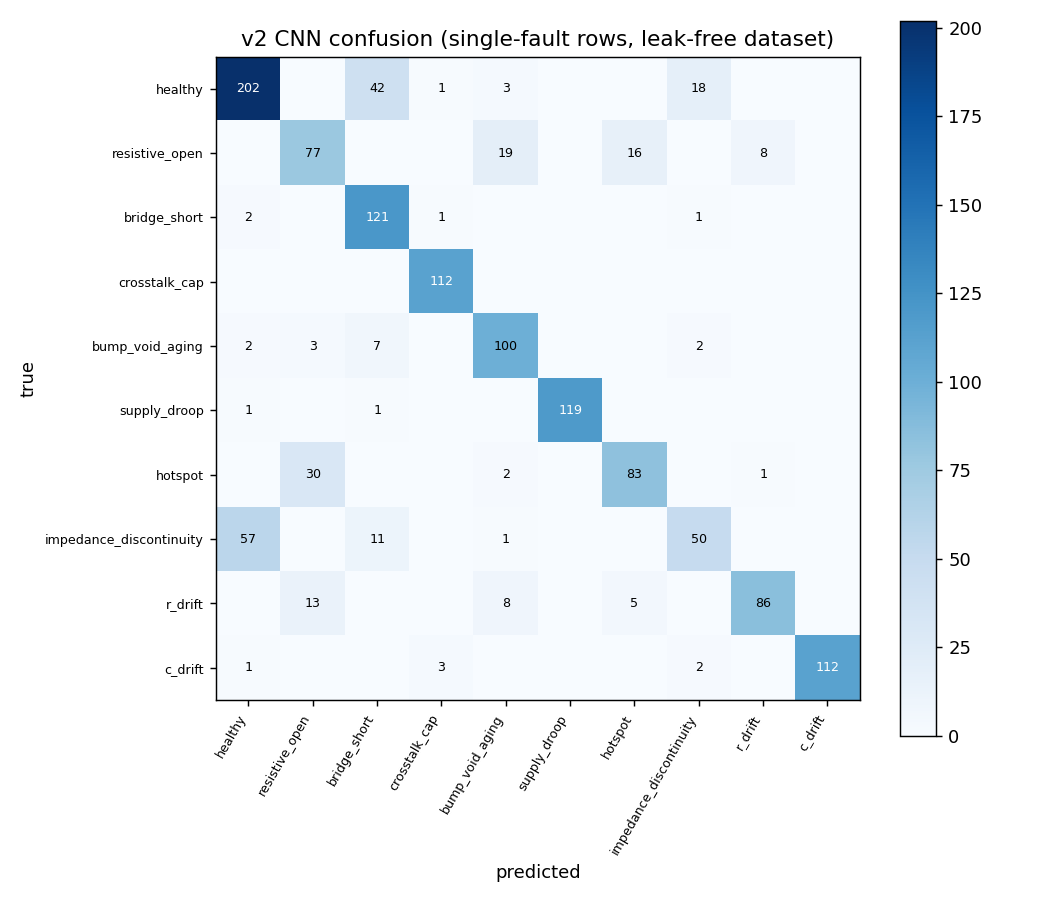
\includegraphics[width=0.62\textwidth]{confusion_v2.png}
\caption{CNN 的混淆矩阵（单故障子集）。残余混淆对应物理上的机制简并：近标称阻抗台阶$\approx$健康、
热点$\approx$局部串阻、两类凸点／导线串阻故障在重叠幅度区间不可分。}\label{fig:confusion}
\end{figure}

\subsection{多标签诊断与码型泛化}\label{sec:v2ml}
多标签头用 9 个独立的 sigmoid 位替代 softmax 十分类，以覆盖并发故障；判决阈值在验证集上
按每类 F1 校准（带类权重的 BCE 训练使 sigmoid-0.5 不再是合理工作点，这与生产监测器需要
标定报警阈值是同一件事）。结果见表~\ref{tab:v2ml}，有三个观察。

\textbf{其一}，多标签设定再次拉开学习模型与线性基线的差距：逻辑回归完全匹配（exact-match，9 个
故障位全对）仅 0.001，CNN 达 0.54--0.59、宏平均 F1（macro-F1）0.72——两处故障沿分布参数信道级联、
其对端到端响应的作用以二端口形式耦合（非两单故障波形的线性相加），合成征象非两者之和，线性模型
无法以独立线性位将其解耦。\textbf{其二}，码型泛化成立且不依赖显式条件输入：在完全未见过的 PRBS 种子上测试，仅读
波形的 CNN 完全匹配为 0.581，与随机划分的 0.542 相当——跨随机码型训练本身已使模型学到码型不变的
故障特征；把理想发送波形作为第二输入通道（发送条件）没有带来一致增益（随机划分 0.526，未见码型
0.513），故随机化训练码型即足以获得码型不变性，显式条件输入在本设定下不必要。\textbf{其三}，健康
误报率在多标签头下偏高（0.39--0.74）：它是 9 个按各自 F1 校准的检测位的并集——每个位为照顾少数类
检出而牺牲特异性，9 个位的误报在健康样本上累积。这提示部署形态应当是分层的：先用二分类健康门
（表~\ref{tab:tele} 的检测器，融合遥测后健康误报 0.094）判断是否异常，再用多标签头做根因归属，
而非直接取多标签并集作为报警。

\begin{table}[h]\centering\small
\caption{多标签诊断（阈值经验证集校准）。exact（完全匹配）= 9 个故障位全对的样本比例；健康 FA（误报，false alarm）=
健康样本被至少一个位报警的比例；故障检出 = 故障样本被至少一个位命中的比例。发送条件 =
以理想发送波形为第二输入通道。未见码型 = 测试集仅含训练中未出现的 PRBS 种子}\label{tab:v2ml}
\begin{tabular}{@{}llcccc@{}}
\toprule
划分 & 模型 & exact & macro-F1 & 健康 FA & 故障检出 \\
\midrule
随机 & 逻辑回归（波形） & 0.001 & 0.278 & 1.000 & 1.000 \\
随机 & CNN（波形） & 0.542 & 0.718 & 0.556 & 0.926 \\
随机 & CNN（波形+发送条件） & 0.526 & 0.723 & 0.707 & 0.935 \\
随机 & CNN（+发送条件+遥测） & \textbf{0.592} & \textbf{0.725} & 0.508 & 0.903 \\
未见码型 & CNN（波形） & 0.581 & 0.717 & 0.390 & —— \\
未见码型 & CNN（波形+发送条件） & 0.513 & 0.713 & 0.739 & —— \\
\bottomrule
\end{tabular}
\end{table}

\subsection{严重度回归}
\begin{table}[h]\centering\small
\caption{连续漂移故障的严重度回归（单故障子集）。MAE 为平均绝对误差（mean absolute error）}\label{tab:sev}
\begin{tabular}{@{}lccc@{}}
\toprule
故障 & 归一化 MAE & $R^2$ & $n_\text{test}$ \\
\midrule
r\_drift（分布式串阻） & 0.076 & 0.894 & 112 \\
c\_drift（并联电容） & 0.071 & 0.908 & 118 \\
\bottomrule
\end{tabular}
\end{table}

两类连续漂移的严重度都可从波形回归到 $R^2\approx0.9$（归一化 MAE 约 0.07）——且这是在信道制造偏差、
发送抖动与随机码型三类滋扰全部存在的条件下取得的，说明波形确实携带连续的退化程度信息，而非仅携带
类别。\texttt{r\_drift} 略低于 \texttt{c\_drift}（0.894 对 0.908），其相对差可归于分布式串阻与温度（经
$R_\text{on}(T)$）在波形上近乎共线、构成一个仅凭波形难以分辨的子空间——这部分残差须由遥测提供正交
约束方能压缩（即下一小节遥测价值的根源）；两者共同的 $R^2$ 缺口则主要是回归的一般残差。

\subsection{遥测消融：多模态融合的价值取决于观测的有损性}\label{sec:tele}
\paragraph{本实验考察的问题。} 本小节回答“在什么条件下，融合温度／供电跌落这类环境遥测才有用”，
这是观测与数据融合的问题，与“为什么需要学习模型”（第~\ref{sec:why} 节）正交。需说明，温度闭合眼图
源于 $R_\text{on}(T)$ 随温度上升（§3.5），是有物理依据的真实机制而非为制造结论而设的数据构造；本
实验只是把该混杂显式建进仿真，再问主观测有损时遥测能否将其扣除。

\begin{table}[h]\centering\small
\caption{遥测消融：A（仅信号）对 B（信号 + 温度／供电跌落），两种观测体制。完整波形为 CNN 十分类
（单故障子集）；有损体制为眼裕度标量上的逻辑回归二分类（全部样本）。“高应力健康 FA”指温度
$\geq85^\circ$C 或供电跌落 $\geq5\%$ 的健康测试样本被误报的比例}\label{tab:tele}
\begin{tabular}{@{}llccc@{}}
\toprule
观测体制 & 方法 & 准确率 & 健康 FA & 高应力健康 FA \\
\midrule
完整波形 & A 仅波形 & 0.789 & 0.237 & 0.281 \\
完整波形 & B +遥测 & \textbf{0.803} & 0.241 & 0.222 \\
有损标量 & A 仅裕度 & 0.708 & 0.361 & 0.492 \\
有损标量 & B 裕度+遥测 & \textbf{0.750} & \textbf{0.094} & \textbf{0.093} \\
\bottomrule
\end{tabular}
\end{table}

当训练分布覆盖部署工况、且混杂效应不与任一故障类的波形签名共线时，完整波形近似为混杂变量（温度／
供电跌落）的充分统计量：给定波形后标签与遥测近乎条件独立，故遥测近乎无增量信息（$0.789\to0.803$）。
该充分性有条件——训练覆盖不足（温度外推，\S\ref{sec:tempholdout}）或混杂与故障类共线（翘曲，
\S\ref{sec:mechresult}）时即失效，遥测重新变得必要。单一眼裕度标量则不是充分统计量，它把不同
（根因，温度）组合压到同一裕度值，丢失的混杂维度须由遥测补回，于是良性高应力
链路与真实故障在该标量上重叠（图~\ref{fig:lossy}）：单看裕度时高应力健康链路有 49\% 被误报，加入
温度／供电跌落后该误报率降到 9\%（检出率不变，$0.723$ 对 $0.716$）。这正是多模态融合在 D2D 在役
监测中的价值边界——且因温度对所有类别同分布采样（\S\ref{sec:dataset}），不存在“某温度只有健康”的
捷径，该增益只能来自对 $R_\text{on}(T)$ 混杂的显式扣除。

\begin{figure}[h]\centering
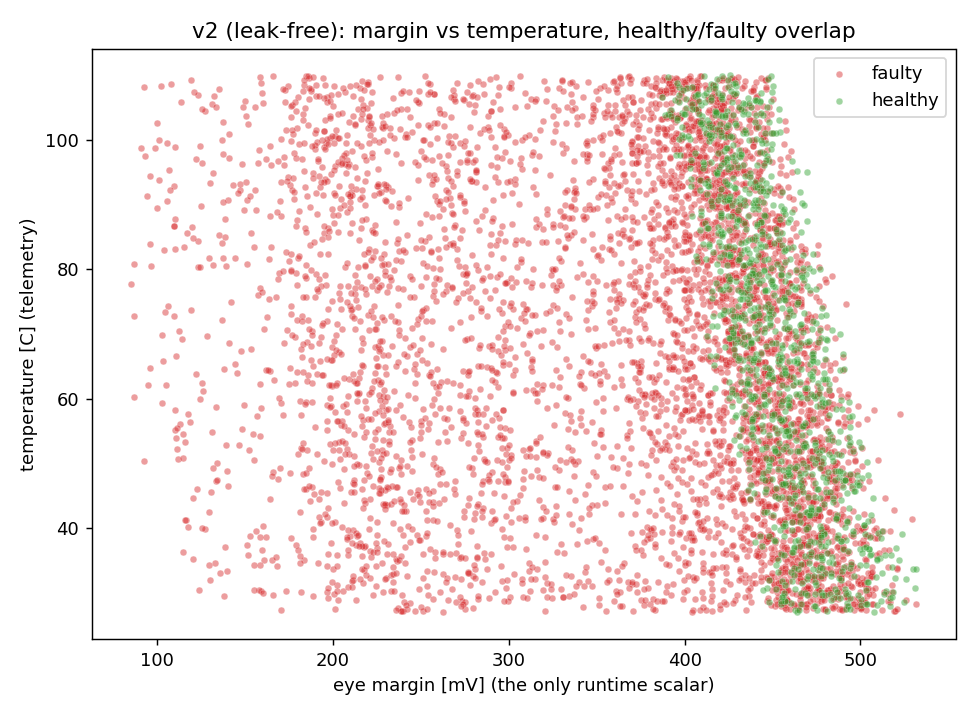
\includegraphics[width=0.6\textwidth]{lossy_confounder_v2.png}
\caption{有损观测下的混杂。横轴是运行时唯一可得的眼裕度标量，纵轴是温度遥测。健康（绿）与故障
（红）在裕度轴上大范围重叠，且健康样本的裕度随温度整体左移（$R_\text{on}(T)$ 闭眼）——任何单一
裕度阈值都无法在不误报高温健康链路的前提下保住检出率；加入温度这一维后，“裕度低但温度高”的
样本可被正确解释为良性。}\label{fig:lossy}
\end{figure}

\subsection{区域消融：判别信息住在波形何处}
\begin{table}[h]\centering\small
\caption{区域消融（区域掩膜逐样本由其发送比特生成，区域外置零；3 次重初始化，均值$\pm$标准差）}\label{tab:region}
\begin{tabular}{@{}lc@{}}
\toprule
训练所用区域 & 准确率 \\
\midrule
全波形 & $0.752\pm0.011$ \\
仅沿区 & $0.749\pm0.009$ \\
仅平台区 & $0.649\pm0.036$ \\
\bottomrule
\end{tabular}
\end{table}

两个结论（图~\ref{fig:region}）。\textbf{其一，判别信息主要集中在跳变沿区}：仅保留沿区与全波形统计
上不可区分（$0.749$ 对 $0.752$），而仅保留平台区准确率降约 10 个百分点（$0.649$）、标准差升至 $0.036$。
机理在于跳变沿是激励中唯一携带高频／瞬态能量的部分，故障对信道传递函数的改变集中在中高频（反射、
ISI、沿斜率皆为频变效应）而只在沿处显现，平台仅承载直流电平；这对观测预算设计有直接含义——按沿
对齐采样优于均匀降采样。\textbf{其二，逐类分解暴露了反射域故障的观测依赖}：\texttt{impedance\_discontinuity}
在仅平台区下准确率降至 $0.03$（沿区 $0.40$）——阻抗台阶的征象是跳变沿处的反射回波，平台上几乎无迹
可寻，与 \S\ref{sec:faultdef} 的电学分析一致；\texttt{resistive\_open}（$0.58\to0.31$）与 \texttt{r\_drift}
（$0.67\to0.51$）同样依赖沿区。反向的例外是健康类（平台区 $0.76>$ 沿区 $0.59$）：健康样本的判别证据
恰是“平台干净、电平正确”。表中全波形均值 $0.752$ 略低于表~\ref{tab:diag} 的 $0.789$（后者为单次训练，
本表为 3 次重初始化均值），区域间比较以本表内部为准。

\begin{figure}[h]\centering
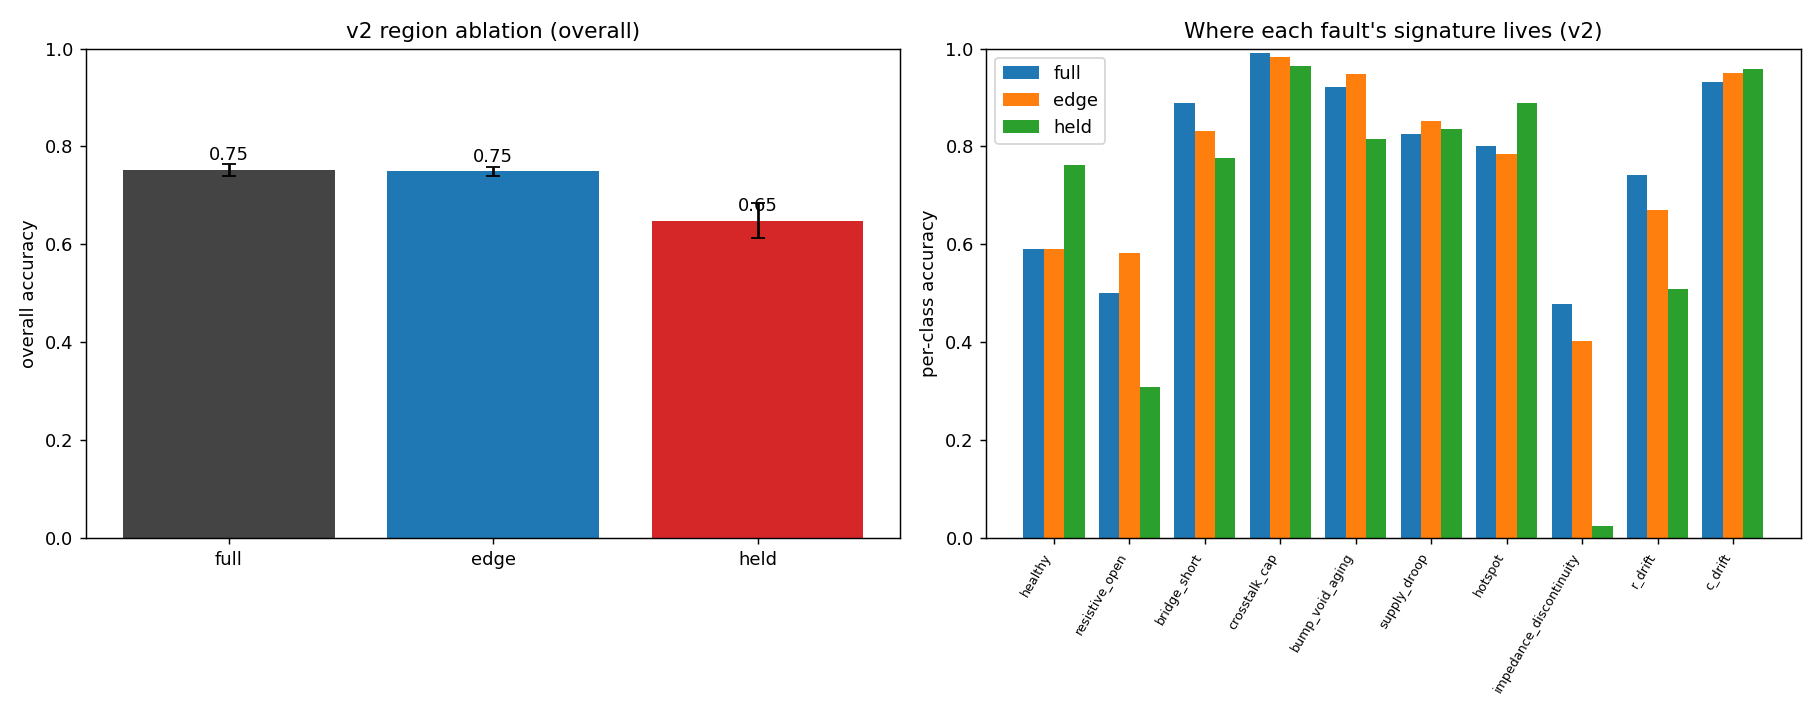
\includegraphics[width=0.95\textwidth]{region_ablation_v2.png}
\caption{区域消融。左：总体准确率（3 次重初始化，误差棒为标准差）；右：逐类准确率——
\texttt{impedance\_discontinuity} 在仅平台区下降至 $0.03$，健康类反而在平台区更高。}\label{fig:region}
\end{figure}

\subsection{开集检测：一个诚实的负结果}\label{sec:openset}
在役监测会遇到训练时未见过的故障模式。我们做留一类实验：将某故障类整体从训练集移除，用最大
softmax 概率（max-softmax）置信度判断测试样本是否属于“未知类”。结果是负面的：留出的
\texttt{bridge\_short} 未知检测的受试者工作特征曲线下面积（area under the ROC curve, AUROC）仅
0.622，\texttt{hotspot} 0.559，\texttt{c\_drift} 仅 0.303（未知样本反而更自信——被高置信地归入形状
相近的已知类）。其本质是：闭集 softmax 把特征空间穷尽划分为已知类的决策区域，并无“已知之外”的
概率质量，置信由类间 logit 差（而非到训练流形的距离）决定，落入某已知决策区的未知样本会被任意高
置信吸收，交叉熵的外推更使远离流形处仍输出尖峰（校准失效）；因此分类置信度天然无法表达“未知”。
可靠的在役系统需要显式的分布外检测（如基于重构误差或密度估计），列为后续工作。

\subsection{补充消融一：温度留出——模型不是在背仿真模板}\label{sec:tempholdout}
主实验全部采用按类分层的随机 75/25 划分，训练与测试共享温度支撑，不能排除“模型只是记住了各温度
下的仿真模板”这一解释。本实验把整段温度区间从训练集\textbf{完全移除}（设置与表~\ref{tab:tele}
完整波形行一致：单故障十分类、双通道 CNN、逆频率类权重；归一化统计仅取自训练行）：

\begin{table}[h]\centering\small
\caption{温度留出。插值带 = 训练 $T<60$ 或 $T\geq85^\circ$C、测试 $60\leq T<85^\circ$C；
外推带 = 训练 $T<85^\circ$C、测试 $T\geq85^\circ$C。基线为随机划分（表~\ref{tab:tele}）}\label{tab:tempholdout}
\begin{tabular}{@{}llccc@{}}
\toprule
划分 & 方法 & 准确率 & 健康 FA \\
\midrule
随机（基线） & A 仅波形 & 0.789 & 0.237 \\
随机（基线） & B +遥测 & 0.803 & 0.241 \\
插值带 & A 仅波形 & 0.806 & 0.216 \\
插值带 & B +遥测 & 0.815 & 0.163 \\
外推带 & A 仅波形 & 0.691 & 0.734 \\
外推带 & B +遥测 & \textbf{0.770} & \textbf{0.399} \\
\bottomrule
\end{tabular}
\end{table}

两个结论。\textbf{其一，插值无性能损失}：在未见过的 $60$--$85^\circ$C 中段上，准确率与随机划分持平
（$0.806/0.815$ 对 $0.789/0.803$）——模型学到的是随温度连续变化的物理规律而非逐温度模板。
\textbf{其二，外推暴露了遥测的第二个价值点}：外推到未见过的高温带时，仅波形模型把 $73\%$ 的健康样本
误报为故障（未见过的高温眼形超出健康流形），加遥测后准确率回到 $0.770$、误报近乎减半——在温度支撑
外推时，遥测在完整波形体制下也不再冗余。这把 \S\ref{sec:tele} 的结论精化为：“遥测冗余”成立的前提是
训练分布覆盖了部署工况；覆盖不足时遥测是波形之外必要的外推锚点。

\subsection{补充消融二：遥测传感器噪声——融合的收益不依赖完美传感器}\label{sec:telnoise}
表~\ref{tab:tele} 的“误报 $49\%\to9\%$”用的是理想真值遥测；真实 DTS 有 $\pm1$--$3^\circ$C 误差与
$1^\circ$C 量化，供电跌落监测器按周期采样供电轨、可能漏掉部分跌落深度。本实验给有损体制的遥测加噪
（训练与测试都加噪——传感器永远有噪；$T_\text{tel}=\mathrm{round}(T+\mathcal N(0,\sigma_T))$，
$d_\text{tel}=\max(0,\,d\cdot u+\mathcal N(0,\sigma_v))$，欠采样变体 $u\sim U(0.6,1)$ 模拟监测器
只捕获 $60$--$100\%$ 的真实跌落）：

\begin{table}[h]\centering\small
\caption{遥测噪声扫描（有损体制，裕度+遥测逻辑回归；3 个噪声/训练种子，均值$\pm$标准差）。
无遥测基线：健康 FA $0.361$、高应力健康 FA $0.492$}\label{tab:telnoise}
\begin{tabular}{@{}lccc@{}}
\toprule
传感器模型 & 健康 FA & 高应力健康 FA & 故障检出 \\
\midrule
理想真值 & $0.039\pm0.040$ & $0.036\pm0.041$ & $0.658$ \\
$\sigma_T{=}1^\circ$C, $\sigma_v{=}0.5\%$ & $0.035\pm0.035$ & $0.038\pm0.040$ & $0.653$ \\
$\sigma_T{=}2^\circ$C, $\sigma_v{=}1\%$ & $0.055\pm0.045$ & $0.071\pm0.057$ & $0.652$ \\
$\sigma_T{=}5^\circ$C, $\sigma_v{=}2\%$ & $0.081\pm0.063$ & $0.109\pm0.087$ & $0.657$ \\
欠采样供电跌落（$u\sim U(0.6,1)$） & $0.095\pm0.080$ & $0.114\pm0.098$ & $0.667$ \\
\midrule
训练用真值、部署遇噪声（$2^\circ$C/$1\%$） & $0.150$ & $0.155$ & $0.717$ \\
\bottomrule
\end{tabular}
\end{table}

结论：\textbf{融合收益对传感器噪声平滑退化}——即便 DTS 误差放大到 $5^\circ$C、供电跌落监测器
只捕获六成跌落，高应力健康误报仍在 $11\%$ 量级，远低于无遥测的 $49\%$；检出率全程稳定。
两个提醒：(i) 失配比噪声影响更大——训练用真值、部署才遇到噪声时误报升至 $15\%$（约 $3\times$），
故训练时就应注入传感器噪声；(ii) 本表为 3 种子均值，种子间标准差约 $\pm0.04$，与表~\ref{tab:tele}
的单次 $9.4\%$ 同量级。完整波形体制下的对照（CNN+噪声遥测，$2^\circ$C/$1\%$）准确率 $0.795$ 对干净
遥测 $0.803$——遥测在该体制本就近乎冗余，加噪几乎无影响。

\subsection{补充消融三：逐类可分性——哪些故障真的可分}\label{sec:perclass}
宏平均会掩盖“哪些类真的可分、哪些只是衰减类之间互相混淆”。对表~\ref{tab:tele} 的 B 设置
（CNN+遥测，单故障测试行）做逐类分解（图~\ref{fig:perclass}），可分性清晰地分成三档：

\begin{itemize}
\item \textbf{最高档（F1 $\geq0.97$）}：\texttt{supply\_droop}（0.992）、\texttt{crosstalk\_cap}
（0.978）、\texttt{c\_drift}（0.974）——各自的眼图签名（全局摆幅缩、跳变沿模糊、沿斜率变缓）
在波形上唯一，与衰减类正交。
\item \textbf{良好（F1 $0.76$--$0.83$）}：\texttt{r\_drift}（0.831）、\texttt{bump\_void\_aging}
（0.810）、\texttt{bridge\_short}（0.788）、\texttt{hotspot}（0.755）、\texttt{healthy}（0.761）。
\item \textbf{薄弱}：\texttt{impedance\_discontinuity}（F1 $0.521$、召回仅 $0.420$）与
\texttt{resistive\_open}（0.634）。
\end{itemize}

前 5 大混淆对印证了眼图签名族的预测：\texttt{impedance\_discontinuity}$\to$\texttt{healthy}（57 例，最大
单项错误——反射征象只住在跳变沿的回波里，幅度域近乎不可见，与区域消融的 $0.03$ 一致）；
\texttt{healthy}$\to$\texttt{bridge\_short}（42）；以及衰减族内部的三角互混
\texttt{hotspot}$\to$\texttt{resistive\_open}（30）、\texttt{resistive\_open}$\to$
\texttt{bump\_void\_aging}（19）、\texttt{r\_drift}$\to$\texttt{resistive\_open}（13）——四个衰减类
共享“串联电阻升高 $\to$ 幅度下降”这一种机理，位置与时间常数的差异只剩二阶线索。把 10 类折叠成
5 个眼图签名族后准确率 $0.803\to0.883$，全部错误中 $41\%$ 留在同族之内：根因定位到“机理族”粒度
是可靠的，族内的精细区分（哪个串阻类）才是剩余难点——这正是 \S\ref{sec:rootcause} 建议把根因输出
与维修动作（重路由／重训练均衡器／降频）绑定的原因：同族故障的维修动作本就相同。

\begin{figure}[h]\centering
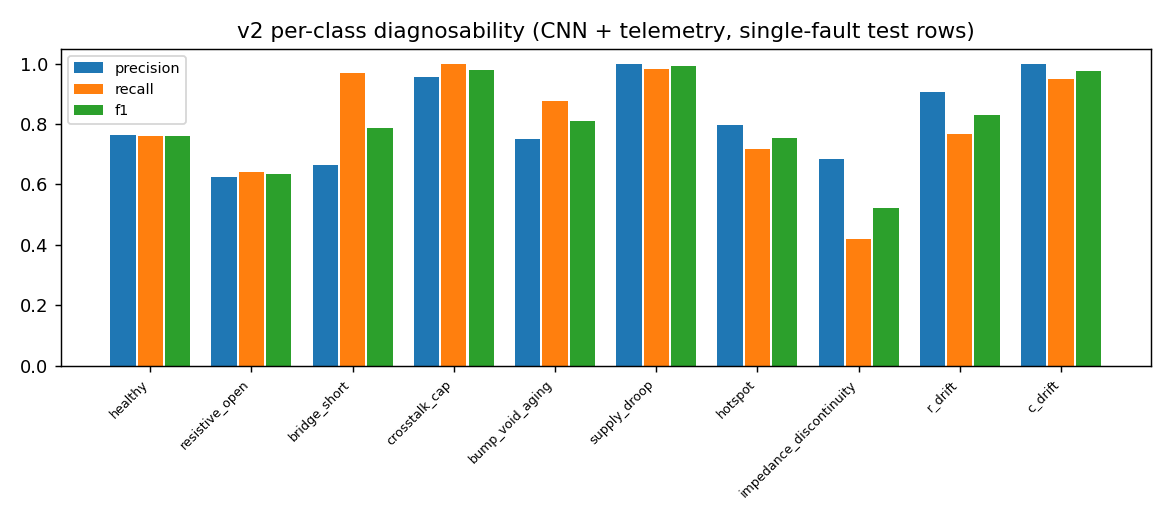
\includegraphics[width=0.95\textwidth]{per_class_v2.png}
\caption{逐类精确率／召回率／F1（CNN+遥测，单故障测试行）。三档可分性：供电跌落／串扰／\texttt{c\_drift}
为最高档；衰减族内部互混；\texttt{impedance\_discontinuity} 召回降至 0.420（57 例漏为 \texttt{healthy}）。}
\label{fig:perclass}
\end{figure}

\subsection{补充实验四：机械轴（v3）——翘曲混杂使仅波形诊断准确率降 7 个百分点、误报翻倍，
温度／供电跌落遥测即可恢复}\label{sec:mechresult}
在 \S\ref{sec:mech} 的 v3 数据集（6000 条、零仿真失败；翘曲 $w\sim U(0,150)\,\mu$m，三路遥测）上
重复遥测消融。完整波形体制为 3 个训练种子的均值$\pm$标准差；v2 基线为单次训练：

\begin{table}[h]\centering\small
\caption{v3 机械混杂下的遥测消融（完整波形 CNN 十分类，单故障子集）。“高翘曲健康 FA”指翘曲应力
分量 $\sigma_w\geq150$\,MPa（约 $w\geq100\,\mu$m）的健康测试样本被误报的比例}\label{tab:mech}
\begin{tabular}{@{}lcccc@{}}
\toprule
设置 & 遥测 & 准确率 & 健康 FA & 高翘曲健康 FA \\
\midrule
v2 基线 A & 无 & 0.789 & 0.237 & --- \\
v2 基线 B & $T$+跌落 & 0.803 & 0.241 & --- \\
\midrule
v3 A 仅波形 & 无 & $0.721\pm0.030$ & $0.543\pm0.133$ & $0.594\pm0.131$ \\
v3 B2 & $T$+跌落 & $0.789\pm0.016$ & $0.328\pm0.074$ & $0.394\pm0.096$ \\
v3 B & $T$+跌落+应力 & $0.785\pm0.011$ & $0.310\pm0.068$ & $\mathbf{0.285\pm0.064}$ \\
\bottomrule
\end{tabular}
\end{table}

三个发现。\textbf{其一，机械混杂使仅波形诊断准确率下降、稳定性降低}：与 v2 相比，加入翘曲后仅波形
准确率降 7 个百分点（$0.789\to0.721$）、健康误报由 $0.237$ 升至 $0.543$、种子间标准差升至 $\pm0.133$。
原因是签名简并：翘曲的电学效应（角点凸点接触电阻 $0$--$3\,\Omega$、两端）与 \texttt{bump\_void\_aging}
的早期形态（$5\,\Omega$ 起、单端）作用在同一类元件、产生同一种幅度衰减征象——其效应方向在观测流形
上与该故障类近乎共线，波形无法将二者分离；与温度不同（$R_\text{on}(T)$ 的效应是全局形状型，与各故障
方向可分），翘曲在波形上没有独立指纹，“完整波形自带解释”在此失效。\textbf{其二，遥测恢复了诊断，但
起作用的是温度／跌落，而非应力遥测本身}：B2（只加温度／跌落两路）与 B（再加应力路）在准确率与总
健康 FA 上统计不可区分（$0.789$ 对 $0.785$）。解释：应力遥测的 CTE 分量是温度的确定函数
（$2.49$\,MPa/$^\circ$C），对已知温度的模型没有新信息；而翘曲分量虽是新信息，其波形效应有界
（$\leq 2\times3\,\Omega$）——一旦温度／跌落钉住了健康裕度的期望包络，模型可把这条有界的松弛带整体
并入健康流形，无需逐样本知道 $w$。\textbf{其三，应力遥测唯一的（弱）增益恰好出现在它应该出现的地方}：
高翘曲健康样本的误报 B 为 $0.285\pm0.064$、B2 为 $0.394\pm0.096$——方向一致（应力路使误报不再向高
翘曲集中）但 3 种子下不显著。诚实的边界：若翘曲范围与故障注入范围重叠更深（弹性接触电阻进入
$5\,\Omega$ 以上），或建模了主动前端的 n／p 反号应力指纹（\S\ref{sec:mech}），应力遥测应成为承重通道；
在当前耦合强度下它是“有则更稳、无则可由温度／跌落边际化”的冗余通道。

有损体制下结论不变：仅裕度 FA $0.110$（高翘曲健康 $0.163$）、检出 $0.642$；加温度／跌落后
FA 降为 $0$（检出 $0.627$）；再加应力路无增益（检出 $0.604$，种子噪声量级，参见
\S\ref{sec:telnoise} 的 $\pm0.04$）。这给 \S\ref{sec:tele} 的“遥测价值取决于观测有损性”补上第二个
条件：在完整波形体制下，遥测是否冗余还取决于混杂效应在观测流形上是否与某故障类共线——温度不
共线（遥测冗余），翘曲共线（遥测必需）；而具体哪路遥测承重，取决于该混杂能否被已有遥测路边际化。

% =====================================================================
\section{技术分析：AI 为什么是必要的}\label{sec:why}

课程要求重点讨论“AI 为什么有效、以及其局限性”。仅凭 CNN 准确率更高不足以论证“必须用学习模型”——
一个测试工程师会反问：\emph{为什么不用一个眼裕度阈值，或几条人工特征规则？} 本节用三组针对性实验
回答，给出 AI 必要性的可证伪边界。

\paragraph{与上一节的区分。} §\ref{sec:tele} 回答融合问题（遥测何时有用，依赖注入的温度混杂），本节
回答解法问题（为何必须用学习模型）。其中实验二、三不依赖任何注入混杂，只考察“把波形压成固定特征或
单个标量会丢多少可分性”——这是故障物理本身的性质，构成 AI 必要性的主证据；实验一用到该混杂，展示
“混杂存在时一维阈值不够”，其前提是 §\ref{sec:tele} 已论证的物理混杂，本文如实标注这一依赖。

\subsection{实验一：单阈值规则在有损体制下存在结构性的误报-检出权衡}
我们给单阈值规则最大的便利：直接在测试集上枚举所有候选阈值 $\tau$ 选最优（这是任何单阈值规则
的性能上界，即“先知阈值”）。结果（表~\ref{tab:rule}）揭示一个结构性困难：

\begin{table}[h]\centering\small
\caption{有损体制：先知单阈值规则 对 学习的（裕度、温度、供电跌落）边界，均在零误报工作点比较}\label{tab:rule}
\begin{tabular}{@{}lccc@{}}
\toprule
检测器 & 工作点 & 故障检出率 & 健康误报率 \\
\midrule
单阈值规则（先知 $\tau$） & 强制健康误报 = 0 & 0.465 & 0.000 \\
单阈值规则（先知 $\tau$） & 最高准确率点 & $\approx1$ & \textbf{0.974} \\
\textbf{学习边界（裕度+遥测）} & 强制健康误报 = 0 & \textbf{0.611} & \textbf{0.000} \\
\bottomrule
\end{tabular}
\end{table}

解读如下。单阈值规则没有任何工作点能同时做到低误报与高检出：把健康误报压到 0 时故障检出率仅
46.5\%；“最高准确率”点（0.824）的高值仅来自测试集故障占比约 82\%——将几乎所有链路判为故障即可
达到接近基率的准确率（误报率 0.974），不构成可用检测器。根本原因是健康与故障的类条件分布因
$R_\text{on}(T)$ 沿温度滑移、在裕度轴的投影上重叠（图~\ref{fig:lossy}），可分性只存在于（裕度、温度）
联合平面——其分隔面是该平面内的斜边界，而单阈值是垂直于裕度轴的轴对齐超平面，投影后必然重叠，
故数学上无法分隔。

而一个仅多用了温度／供电跌落遥测的学习边界，在同样零误报下把检出率从 46.5\% 提到 61.1\%——严格
优于规则的零误报工作点。这说明此处 AI 的必要性\textbf{不是}“深度网络比线性强”，而是\textbf{问题本身
需要一个多变量决策边界来扣除混杂}，任何固定的单变量规则都做不到。这是一个有判决条件、可证伪的结论。

\subsection{实验二：从原始信号学表征优于固定的人工特征}
表~\ref{tab:diag} 已给出一条三级阶梯：原始波形 + 线性模型 0.221（随机码型下线性模型只剩整体幅度
信息）；18 维码型不变的人工眼图特征 + 逻辑回归／MLP 0.661/0.711（特征工程恢复大部分可分性，但有
信息上限）；原始波形 + CNN 0.789。即把波形压成一组固定的、为单一故障设计的眼图特征会丢信息。区域
消融解释了原因：不同故障的判别信息分布在波形的不同部位，一组固定的少量特征无法同时为所有故障保留
各自依赖位置的统计量；而卷积核在整条波形上滑动、由数据决定关注何处，因而多拿到约 8--13 个百分点。
这正是“从原始信号学表征”相对“经典特征工程”的价值所在，也与课程“不卷模型、看是否真解决问题”的
导向一致——价值来自表征学习覆盖了多类故障，而非堆叠层数。

\subsection{实验三：常规方法只能二分类，学习模型才能给出根因}\label{sec:rootcause}
一个常被陈述的命题是：\emph{常规方法只能判“连接是否有故障”（二分类），而机器学习能进一步分出故障的根因。}
这一命题在本任务中基本成立，但需限定。我们把常规在役监测能拿到的信息——单一眼裕度标量——直接用于
10 类根因判别，与学习模型对比（表~\ref{tab:rootcause}）。

\begin{table}[h]\centering\small
\caption{用不同信息做 10 类根因判别（单故障子集测试集）。多数类基线为 0.201}\label{tab:rootcause}
\begin{tabular}{@{}lc@{}}
\toprule
判别所用信息 & 10 类准确率 \\
\midrule
单一眼裕度标量 & 0.221 \\
眼裕度 + 温度／供电跌落遥测 & 0.204 \\
\textbf{完整波形（CNN）} & \textbf{0.789} \\
\bottomrule
\end{tabular}
\end{table}

眼裕度是从高维波形到标量的多对一投影：串阻、电容、串扰、反射等不同根因被映到同一裕度值的纤维上，
该投影与根因的互信息近乎为零，故单一裕度做 10 类只有 0.221，约等于多数类基线 0.201——它只编码
“眼闭了多少”（健康／故障二分），不编码“被什么闭合”。加上温度／供电跌落遥测也没有改善（0.204）：
遥测正交于根因维、帮的是去混杂（实验一），不增根因信息。而完整波形的形状（沿的快慢、平台的噪声、
反射纹路）保留了区分这些纤维所需的结构，CNN 据此达到 0.789。

因此命题应精确表述为：\textbf{在“有损标量观测”这一常规在役设置下，可得信息只够支撑二分类（且如实验一所示，
连这个二分类在混杂下都不可靠）；要把判别从“是否故障”推进到“何种根因”，须使用保留波形结构的观测 + 学习
模型。}（边界：制造测试中基于确定性图案与故障字典的诊断本可做一定的故障定位，但依赖结构化激励，不适用于
本文在混杂下从单一健康信号做在役参数化诊断的设置。）

\subsection{综合：AI 的必要性边界}
合并三组实验，可以精确陈述 AI 在本任务中“何时必要、何时不必要”：
\begin{itemize}
\item \textbf{当观测有损（运行时标量）且存在混杂}：必须用能表达多变量边界的学习模型来扣除环境共模；
单阈值规则在零误报下损失约 15 个百分点的检出率（0.465 对 0.611）。
\item \textbf{当要从“是否故障”推进到“何种根因”}：单标量裕度的 10 类准确率仅 0.221（约等于多数类
基线水平 0.201），必须用保留波形结构的观测 + 学习模型（CNN 0.789）。这是“常规=二分类、学习=根因”
命题的量化依据。
\item \textbf{当工作负载随机（在役的真实形态）}：原始波形上的线性模型准确率降至 0.221，码型不变的
人工特征达 0.711，学习的卷积表征达 0.789；且结构要匹配信号——同为深度模型的 LSTM 仅 0.249、接近
线性模型水平：起作用的不是“深度”，而是卷积与波形局部平移结构匹配的归纳偏置。
\item \textbf{当观测无损（完整波形）}：波形已隐含混杂变量，额外遥测近乎冗余（$0.789\to0.803$，前提是
训练分布覆盖部署工况且混杂不与故障类共线，否则见 \S\ref{sec:tempholdout}／\S\ref{sec:mechresult}）；此时
“多加遥测总更好”的直觉不成立。这条边界本身就是本文要传达的洞见。
\end{itemize}
% =====================================================================
\section{局限性}

\begin{enumerate}
\item \textbf{匹配良好的短链路对参数／热扰动本征不敏感}：导体电阻远小于驱动+终端，故温度、分布式串阻、热点、
阻抗阶跃在原始眼幅上长期不可见，必须显式引入 $R_\text{on}(T)$、绝对分布式串阻等机制才使其可检。这本身
也是一条物理洞见：单一眼图度量对这类退化的固有灵敏度低。
\item \textbf{阻抗不连续在幅度域几乎不可见}，属反射域故障（混淆矩阵中弱阻抗台阶大量被判为健康），
需 TDR/反射系数模态——进一步印证多模态/多探针的必要性。
\item \textbf{r\_drift 与温度混杂}：分布式串阻与温度同样表现为串阻上升，单波形难以完全分离其严重度
（$R^2$ 0.894，低于无此混杂时的可达水平），需遥测辅助。
\item \textbf{接收端无均衡}：观测取自无源 RX 焊盘（\S\ref{sec:frontend}），不含 CTLE/DFE、判决器失调
与 CDR 抖动。真实接收机的均衡会重塑波形上的故障征象（如部分补偿 \texttt{c\_drift} 的沿变缓），
本文结论严格而言属于“焊盘原始波形”观测体制；迁移到均衡后观测需重新评估。
\item \textbf{仿真数据，缺乏现场标定}：码型/信道/抖动均已随机化，但全部数据仍来自同一仿真器族，
物理参数虽有文献依据，未经实测硅校准；划分为单次分层（区域消融用 3 次重初始化稳健化），
主表数值未做多折交叉验证。
\item \textbf{开集（未知故障）检测无效}：留一类实验（\S\ref{sec:openset}）表明 max-softmax 置信度无法识别
训练未见过的故障类，未知故障会被自信地误判为相近的已知根因——在役部署前必须补充显式的分布外检测。
\item \textbf{多标签健康误报偏高}：9 个按各自 F1 校准的检测位的并集在健康样本上误报累积
（\S\ref{sec:v2ml}），多标签头只宜作根因归属层，报警须由二分类健康门把守。
\end{enumerate}

% =====================================================================
\section{结论与复现}

\subsection{结论}
本项目交付了一个开放、可复现、物理接地的 D2D 互连原始波形故障诊断基准与方法：在码型、信道参数与
发送抖动全部随机化的 6000 样本数据集上，CNN 十分类诊断 78.9\%（融合遥测 80.3\%）、多标签并发故障
诊断 macro-F1 0.72、连续漂移严重度回归 $R^2\approx0.9$。核心贡献是把“多模态遥测是否有用”变成一个有
判决条件的结论——\textbf{其价值取决于主观测的有损性}：完整波形下遥测近乎冗余（$+1.4$ 个百分点）；
有损标量观测下，融合温度／供电跌落把良性高应力误报从 49\% 降到 9\%，并在零误报工作点把检出率从先知
单阈值规则的 46.5\% 提到 61.1\%。配套结论包括：随机工作负载下“从原始信号学习表征”成为必需（原始
波形上的线性模型仅 0.221）、跨码型训练即获码型不变性而无需显式条件输入、以及开集检测的诚实负结果。
这是对“在役 D2D 链路健康多模态融合”空白的问题重构 + 可证伪演示式贡献，而非一个新的机器学习模型。

\subsection{未来工作}
用有损误码序列（比较器位流）替代标量裕度，做时序卷积网络（temporal convolutional network, TCN）
对照；接入 TDR／反射系数模态覆盖阻抗不连续；针对开集负结果引入显式分布外检测（重构误差／密度
估计）；多次交叉验证与实测硅标定。

\subsection{复现说明}
\begin{lstlisting}[language=bash]
cd sim
# 1) 并行生成数据集（8 worker，约 20 min；完整 1 ps 原始波形存 raw/）
~/miniconda3/envs/drl_hw2/bin/python run_wave2.py --out out/wave2 \
    --n-rows 6000 --n-bits 160 --workers 8
# 2) 可视化（带 H/W/BER 标注的眼图、波形、遥测覆盖）
~/miniconda3/envs/drl_hw2/bin/python inspect_waves.py --data out/wave2
# 3) 多标签诊断/码型泛化/遥测消融/开集/严重度回归
~/miniconda3/envs/drl_hw2/bin/python ml_diagnose_v2.py --data out/wave2
# 4) “AI 为什么必要”的基线（先知阈值规则/人工特征/原始波形线性/单标量根因）
~/miniconda3/envs/drl_hw2/bin/python why_ai_v2.py --data out/wave2
# 5) LSTM 对照 + 区域消融
~/miniconda3/envs/drl_hw2/bin/python extra_v2.py --data out/wave2
\end{lstlisting}


% =====================================================================
\begin{thebibliography}{99}\small
\bibitem{huang2024bist} Y.-C. Huang, P.-Y. Lin, J.-F. Li, H.-S. Fu, and Y.-P. Lee,
``Efficient built-in self-test scheme for inter-die interconnects of chiplet-based chips,''
in \emph{Proc. IEEE International Test Conference (ITC)}, 2024.
\bibitem{chuang2025pattern} P.-Y. Chuang, F. Lorenzelli, C.-W. Wu, and E. J. Marinissen,
``Generating test patterns for chiplet interconnects with optimized effectiveness and efficiency,''
\emph{IEEE Trans. Computer-Aided Design of Integrated Circuits and Systems}, vol.~44, no.~3,
pp. 1155--1168, 2025.
\bibitem{wang2024ucie} T.-H. Wang, P.-Y. Chuang, F. Lorenzelli, and E. J. Marinissen,
``Test and repair improvements for UCIe,'' in \emph{Proc. IEEE European Test Symposium (ETS)}, 2024.
\bibitem{cui2023physical} C. Cui, T. Xu, H. Fu, and J. Huang,
``Physical-aware interconnect testing and repairing of chiplets,''
in \emph{Proc. IEEE European Test Symposium (ETS)}, 2023.
\bibitem{huang2018tsv} Y.-J. Huang, S.-C. Lin, C.-L. Pan, and M.-H. Guo,
``Machine-learning approach in detection and classification for defects in TSV-based 3-D IC,''
\emph{IEEE Trans. Components, Packaging and Manufacturing Technology}, vol.~8, no.~4,
pp. 699--706, 2018.
\bibitem{kang2023reflection} T. Y. Kang, H. Lee, and S. Suh,
``Non-destructive fault diagnosis of electronic interconnects by learning signal patterns of
reflection coefficient,'' arXiv:2304.10207, 2023.
\bibitem{medico2018ae} R. Medico, D. Spina, D. Vande Ginste, D. Deschrijver, and T. Dhaene,
``Autoencoding density-based anomaly detection for signal integrity applications,''
in \emph{Proc. IEEE Conf. Electrical Performance of Electronic Packaging and Systems (EPEPS)}, 2018.
\bibitem{usama2026latent} M. Usama, H.-D. Jang, S. Shanbhag, Y.-C. Sung, S.-J. Bae, and D. E. Chang,
``Learning high-quality latent representations for anomaly detection and signal integrity
enhancement in high-speed signals,'' \emph{IEEE Trans. Computer-Aided Design of Integrated
Circuits and Systems}, 2026 (arXiv:2506.18288).
\bibitem{lanzieri2024aging} L. Lanzieri, L. Butkowski, J. Kral, G. Fey, H. Schlarb, and
T. C. Schmidt, ``Switching frequency as FPGA monitor: studying degradation and ageing prognosis
at large scale,'' arXiv:2412.15720, 2024.
\bibitem{ali2020fusion} G. Ali, L. Bagheriye, and H. G. Kerkhoff,
``On-chip embedded instruments data fusion and life-time prognostics of dependable VLSI-SoCs
using machine-learning,'' in \emph{Proc. IEEE Int. Symp. On-Line Testing and Robust System
Design (IOLTS)}, 2020.
\bibitem{ortega2025octane} E. Ortega, A. Hati, J. Talukdar, W. Paik, F. Su, R. Chattopadhyay,
and K. Chakrabarty, ``OCTANE: on-chip telemetry-based anomaly notification engine,''
in \emph{Proc. IEEE International Test Conference (ITC)}, 2025.
\bibitem{zhu2025ice} K. Zhu, D. Huang, L. Costero, and D. Atienza,
``3D-ICE 4.0: accurate and efficient thermal modeling for 2.5D/3D heterogeneous chiplet systems,''
arXiv:2512.05823, 2025.
\bibitem{ma2024cosim} X. Ma, Q. Xu, C. Wang, H. Cao, J. Liu, D. Zhang, and Z. Li,
``An electrical--thermal co-simulation model of chiplet heterogeneous integration systems,''
\emph{IEEE Trans. Very Large Scale Integration (VLSI) Systems}, vol.~32, no.~10,
pp. 1769--1781, 2024.
\bibitem{deric2022puf} A. Deric and D. Holcomb,
``Know time to die -- integrity checking for zero trust chiplet-based systems using between-die
delay PUFs,'' \emph{IACR Trans. Cryptographic Hardware and Embedded Systems (TCHES)}, 2022.
\bibitem{monfared2025quake} S. K. Monfared, M. Saadat Safa, and S. Tajik,
``ChipletQuake: on-die digital impedance sensing for chiplet and interposer verification,''
arXiv:2504.19418, 2025.
\end{thebibliography}

\end{document}
